\section{Simulation}
\label{section:simulation}

\subsection{MAD-X}

\subsection{OPERA model of the MU (I can cite here the IPAC paper)}

\subsection{Explain that it defocuses in H and focuses in V}

\cite{johnson_beam_2022}

\subsection{Kick response (maybe I need more data and MD for this or simply repeat the measurements)}

\subsection{Injection BTP MD}

\subsection{BTP stray elements}

The BTP line has an old model (prior to 2021) that is composed of 233 thin multipole inserted at the end of the transfer line. The model can be accessed via the following links:

\begin{itemize}
    \item \href{https://gitlab.cern.ch/acc-models/acc-models-tls/-/blob/2021/psb_extraction/btp/BTP.ele}{BTP.ele}
    \item \href{https://gitlab.cern.ch/acc-models/acc-models-tls/-/blob/2021/psb_extraction/btp/BTP.seq}{BTP.seq}
\end{itemize}



\subsection{Theory}

The magnetic field \( B_y \) can be expressed as:

\[
B_{y}(x,y) = B_{0} + B_{1}x + B_{2}\frac{1}{2}(x^{2}-y^{2}) + B_{3}\frac{1}{6}(x^{3}-3xy^{2})
\]

where the coefficients \( B_i \) are given by:

\[
B_{i} = K_{i}B\rho
\]

In the old BTP model, the coefficients \( K_{0}, K_{1}, K_{2}, \) and \( K_{3} \) are used.

The relationship for \( K_{0} \) is:

\[
K_{0}L = \frac{B_{0}L}{B\rho}
\]

where 

\[
L = \frac{\text{totalLength}}{\# \text{ elements}}
\]

To extract the pure \( K_{0} \), we divide by \( L \):

\[
K_{0} = \frac{B_{0}}{B\rho}
\]

For tracking, we obtain the field components and divide by \( B\rho \):

\[
B_{0} = K_{0}B\rho
\]

\[
K_{0} = \frac{B_{0}}{B\rho}
\]

The \( K_{1} \) coefficient is computed using two tracks and the relationship:

\[
K_{1} = \frac{\frac{\Delta B_{y}}{\Delta x}}{B\rho}
\]

The \( K_{0}L \) component as a function of \( s \) is shown as follows:

\begin{figure}[H]
\centering
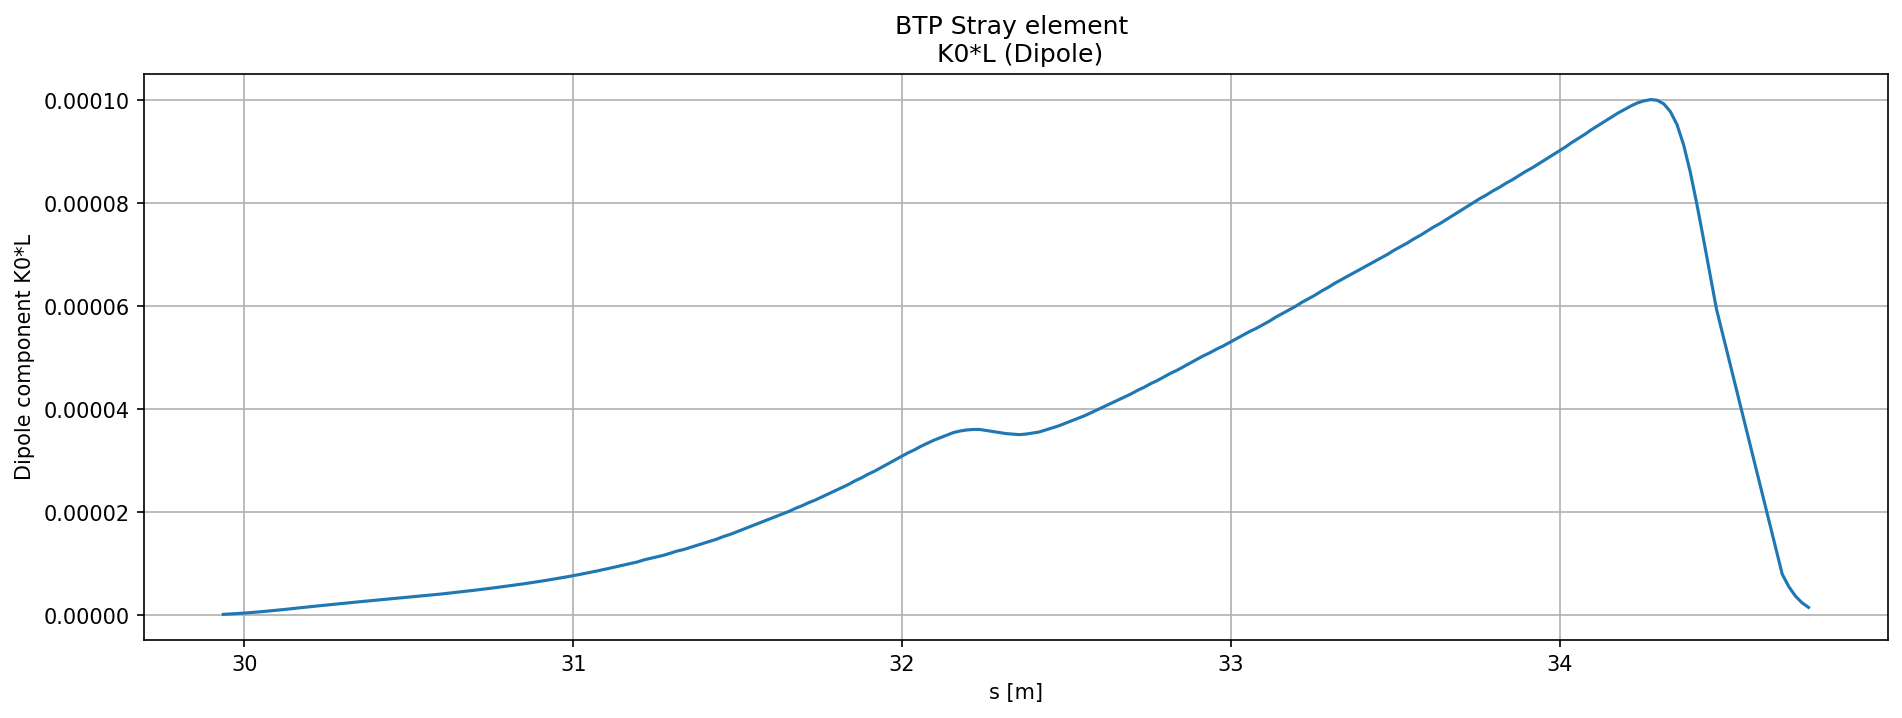
\includegraphics[width=1.0\textwidth]{02_Simulation/images/BTP_old_model_stray.png}
\caption{BTP Stray element old model.}
\label{fig:transfer_matrix_1}
\end{figure}


A goal is to create a multi-component model similar to the old BTP model, first on the BTP line to compare with the old model and then to expand on different injection and extraction that passes through stray fields. The first step is launch particles on the reference track, track them in the stray field magnetic field and probe the B-field perpendicular to the track. Then a 4rd order polynomial is fit for everything position along the injection line, i.e. along different z in meters.

\begin{figure}[H]
\centering
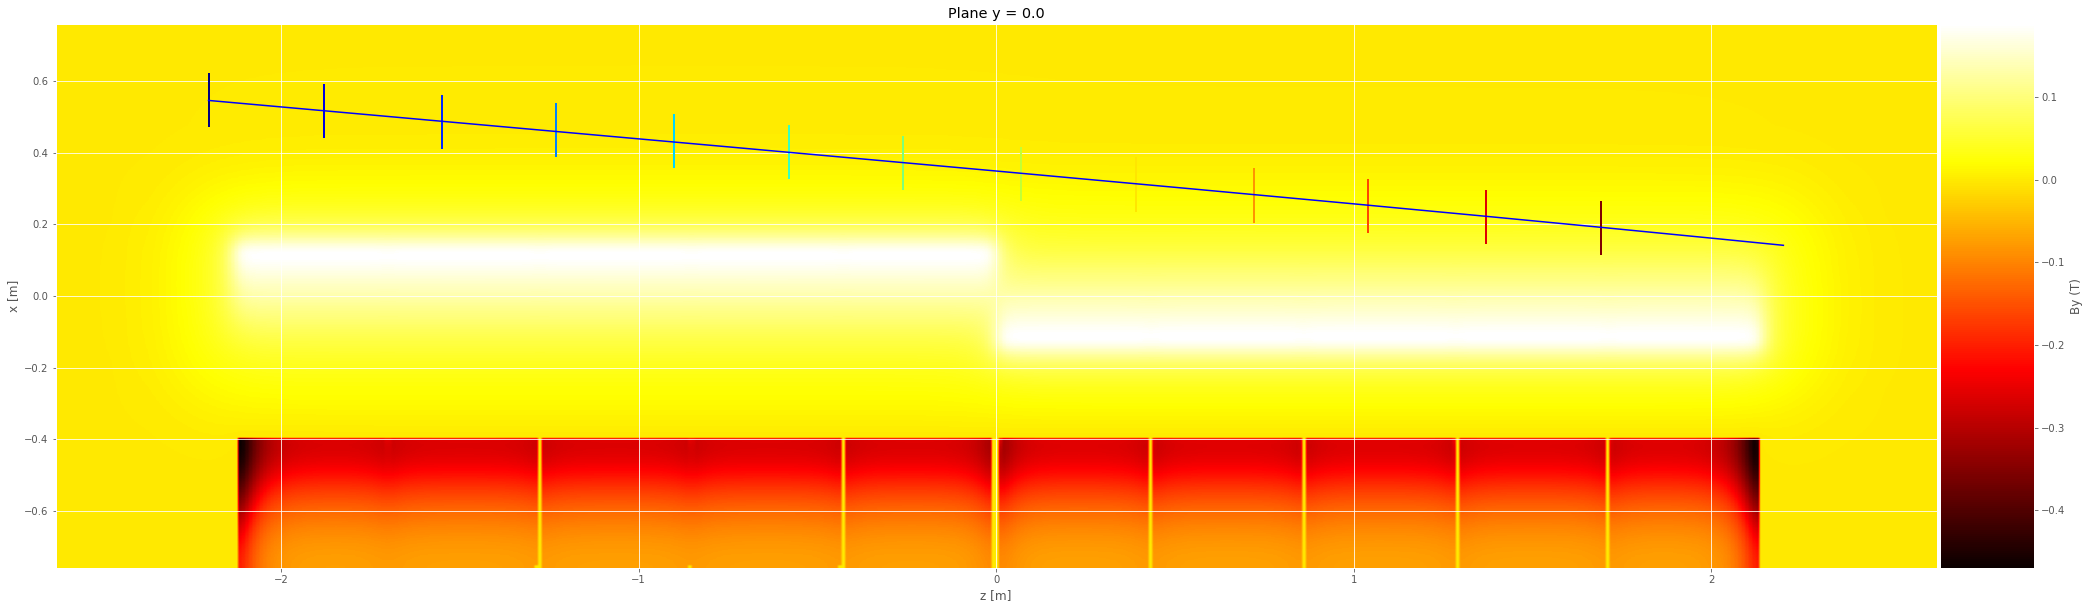
\includegraphics[width=1.0\textwidth]{02_Simulation/images/MCP_track.png}
\caption{Tracking through the MCP injection.}
\label{fig:mcp_track}
\end{figure}

\begin{figure}[H]
\centering
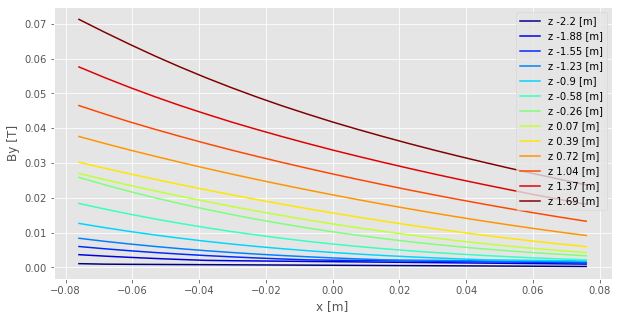
\includegraphics[width=1.0\textwidth]{02_Simulation/images/MCP_track_2.png}
\caption{Probing the B-field tranversly to the injection track.}
\label{fig:mcp_track}
\end{figure}



\begin{figure}[H]
\centering
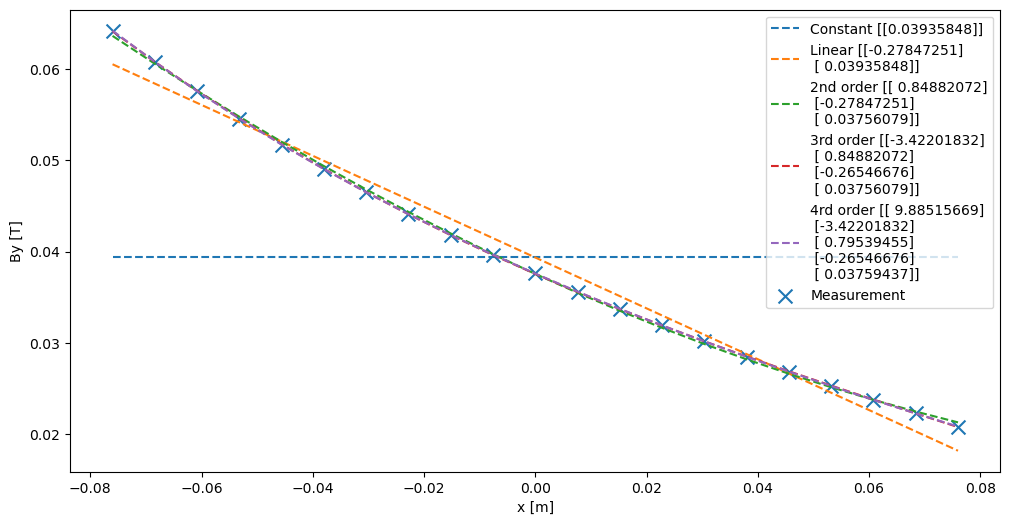
\includegraphics[width=1.0\textwidth]{02_Simulation/images/fit_of_bfield.png}
\caption{.}
\label{fig:fit_bfield}
\end{figure}

\begin{figure}[H]
\centering
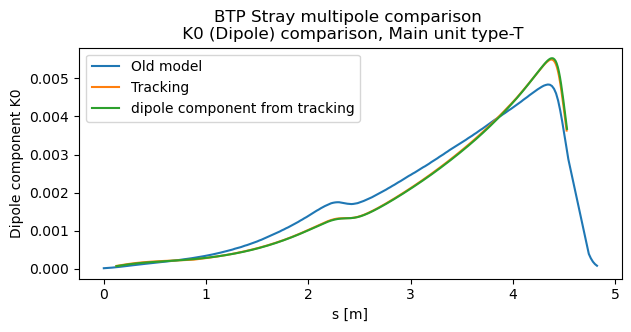
\includegraphics[width=0.7\textwidth]{02_Simulation/images/mcp_dipole.png}
\caption{BTP Stray multipole comparison, K0 (Dipole) comparison, main unit type-T}
\label{fig:mcp_dipole}
\end{figure}

\begin{figure}[H]
\centering
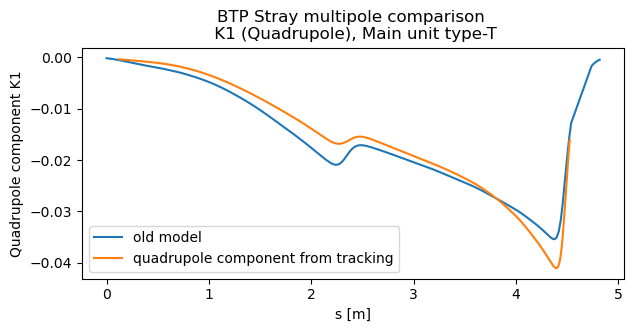
\includegraphics[width=0.7\textwidth]{02_Simulation/images/mcp_quadrupole.png}
\caption{BTP Stray multipole comparison, K1 (Quadrupole) comparison, main unit type-T}
\label{fig:mcp_quadrupole}
\end{figure}

\begin{figure}[H]
\centering
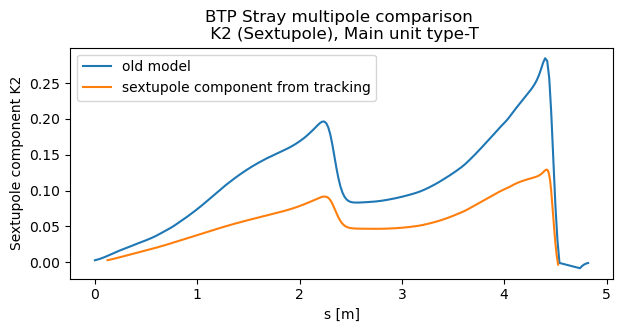
\includegraphics[width=0.7\textwidth]{02_Simulation/images/mcp_sextupole.png}
\caption{BTP Stray multipole comparison, K2 (Sextupole) comparison, main unit type-T}
\label{fig:mcp_sextupole}
\end{figure}

\begin{figure}[H]
\centering
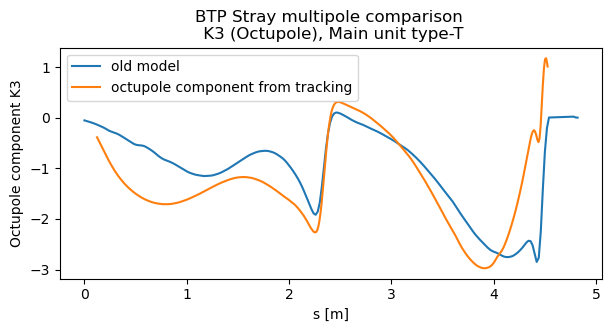
\includegraphics[width=0.7\textwidth]{02_Simulation/images/mcp_octupoles.png}
\caption{BTP Stray multipole comparison, K3 (Octupoles) comparison, main unit type-T}
\label{fig:mcp_quadrupole}
\end{figure}


The code creates MCP models correctly along the s dimension (along the particles track) and transverse along the bend track. For small angles, the difference in dipole component along z or s can be neglected.

\subsection{Multipole field component in MU62}

This section will talk about the multiple field component inside the MU62 main unit which is the magnet that the beam crosses through for the extraction to the East Area.

The following \href{https://gitlab.cern.ch/eljohnso/acc-models-tls-eliott-fork/-/blob/EliottBranch/ps_extraction/east-fast-extraction/mfc_mu62.ipynb}{Notebook: MFC MU62} was used to create the MFC in MU62 using a \SI{24}{\giga\electronvolt\per\clight} beam. Figure \ref{fig:track_mu62} shows the particle track through the stray field of MU62. The initial launching coordinate of the reference particle were \si{0.132}{m} and \si{0.0139}{rad}. The field was probed transversely at discrete s-steps along the particle trajectory inside the vacuum pipe. The vacuum pipe aperture has a total width of \si{70}{mm}. We run a loop for each point in the track we save the $B_{y}$ field perpendicularly to the track  and run a polynomial fit of third order on By as a function of $x_{\perp}$

$$ \alpha = - tan^{-1}\left(\frac{ x_{i}-x_{i-1} } {z_{i}-z_{i-1}} \right)$$

$$ B_{y} = \begin{bmatrix}  
x_{center} + x_{offset}\cdot cos(\alpha_{deflection}) \\  
0 \\
z_{center} + x_{offset}\cdot sin(\alpha_{deflection})
\end{bmatrix} $$



\begin{figure}[H]
\centering
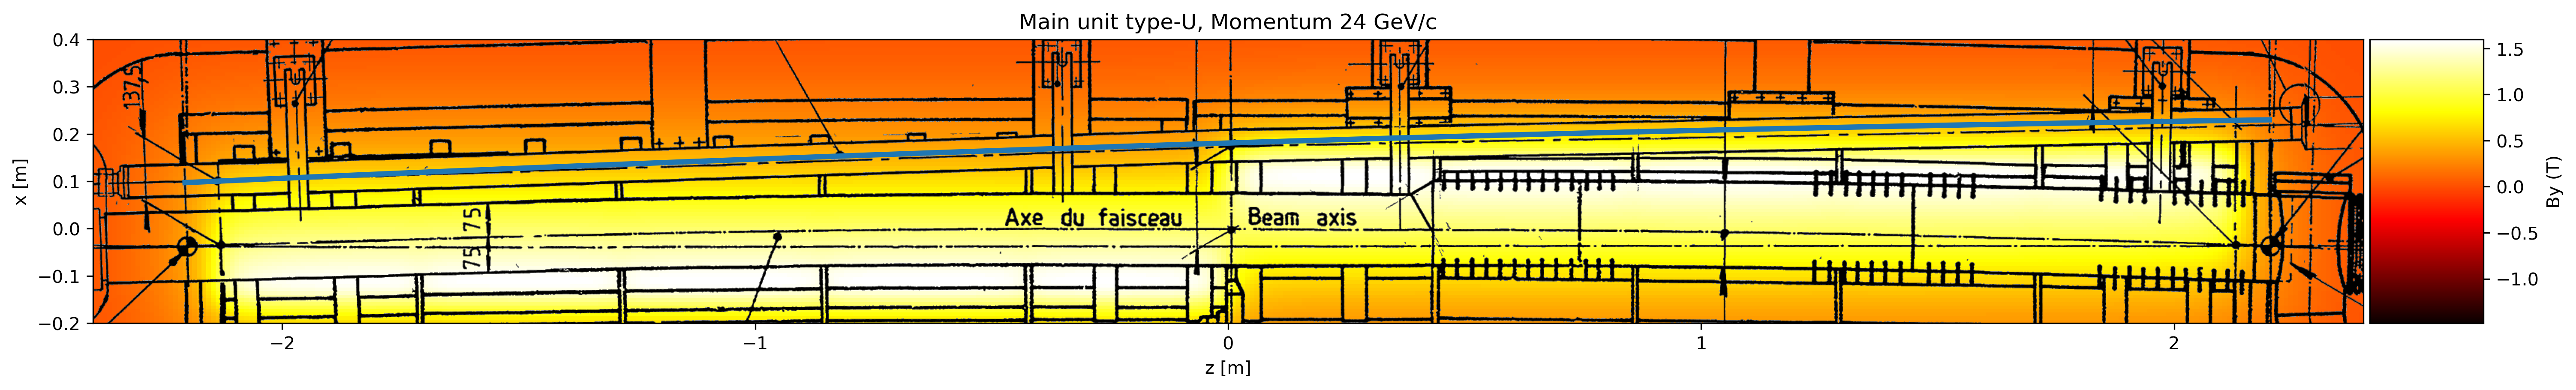
\includegraphics[width=1.0\textwidth]{02_Simulation/images/track_mu62.png}
\caption{Tracking of the proton beam in MU62}
\label{fig:track_mu62}
\end{figure}

\begin{figure}[H]
\centering
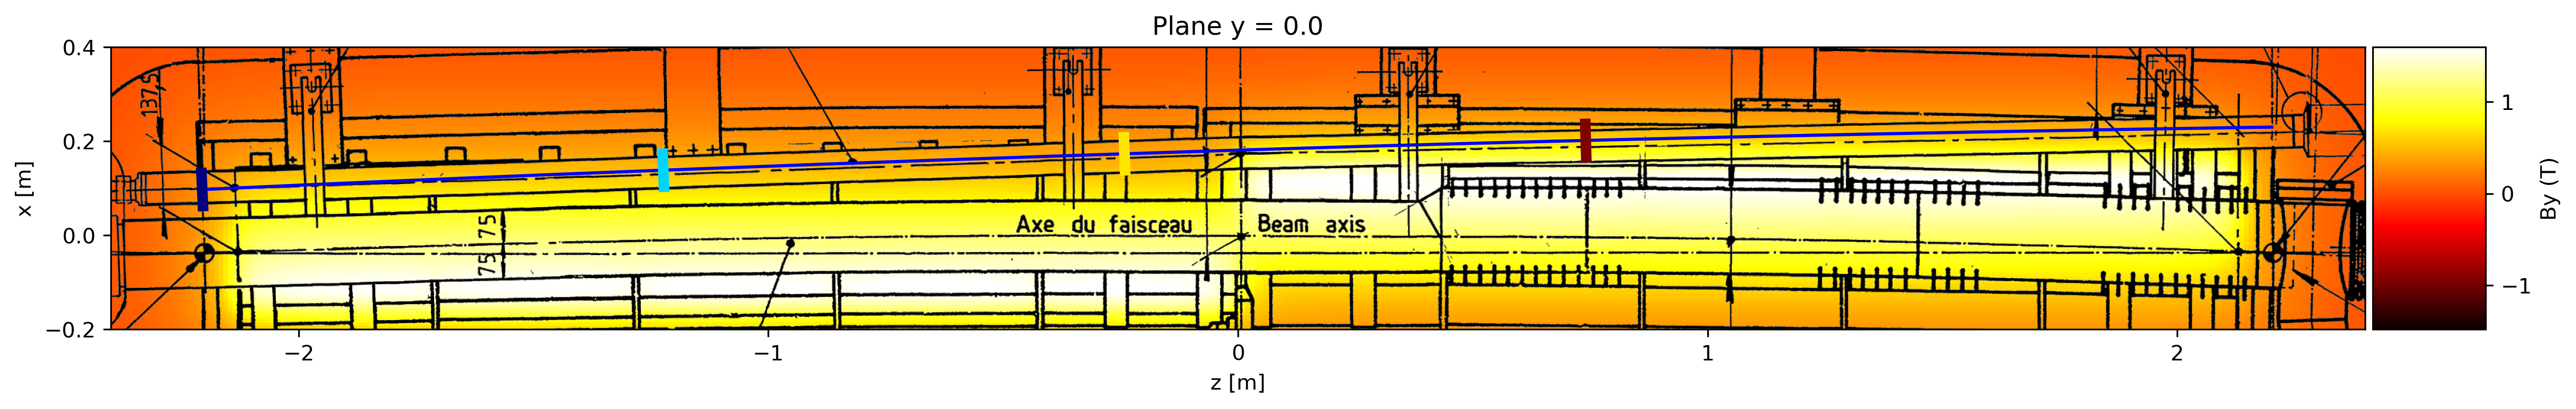
\includegraphics[width=1.0\textwidth]{02_Simulation/images/track_mu62_2.png}
\caption{Tracking of the proton beam in MU62 with example location of MFC sampling}
\label{fig:track_mu62_2}
\end{figure}

\begin{figure}[H]
\centering
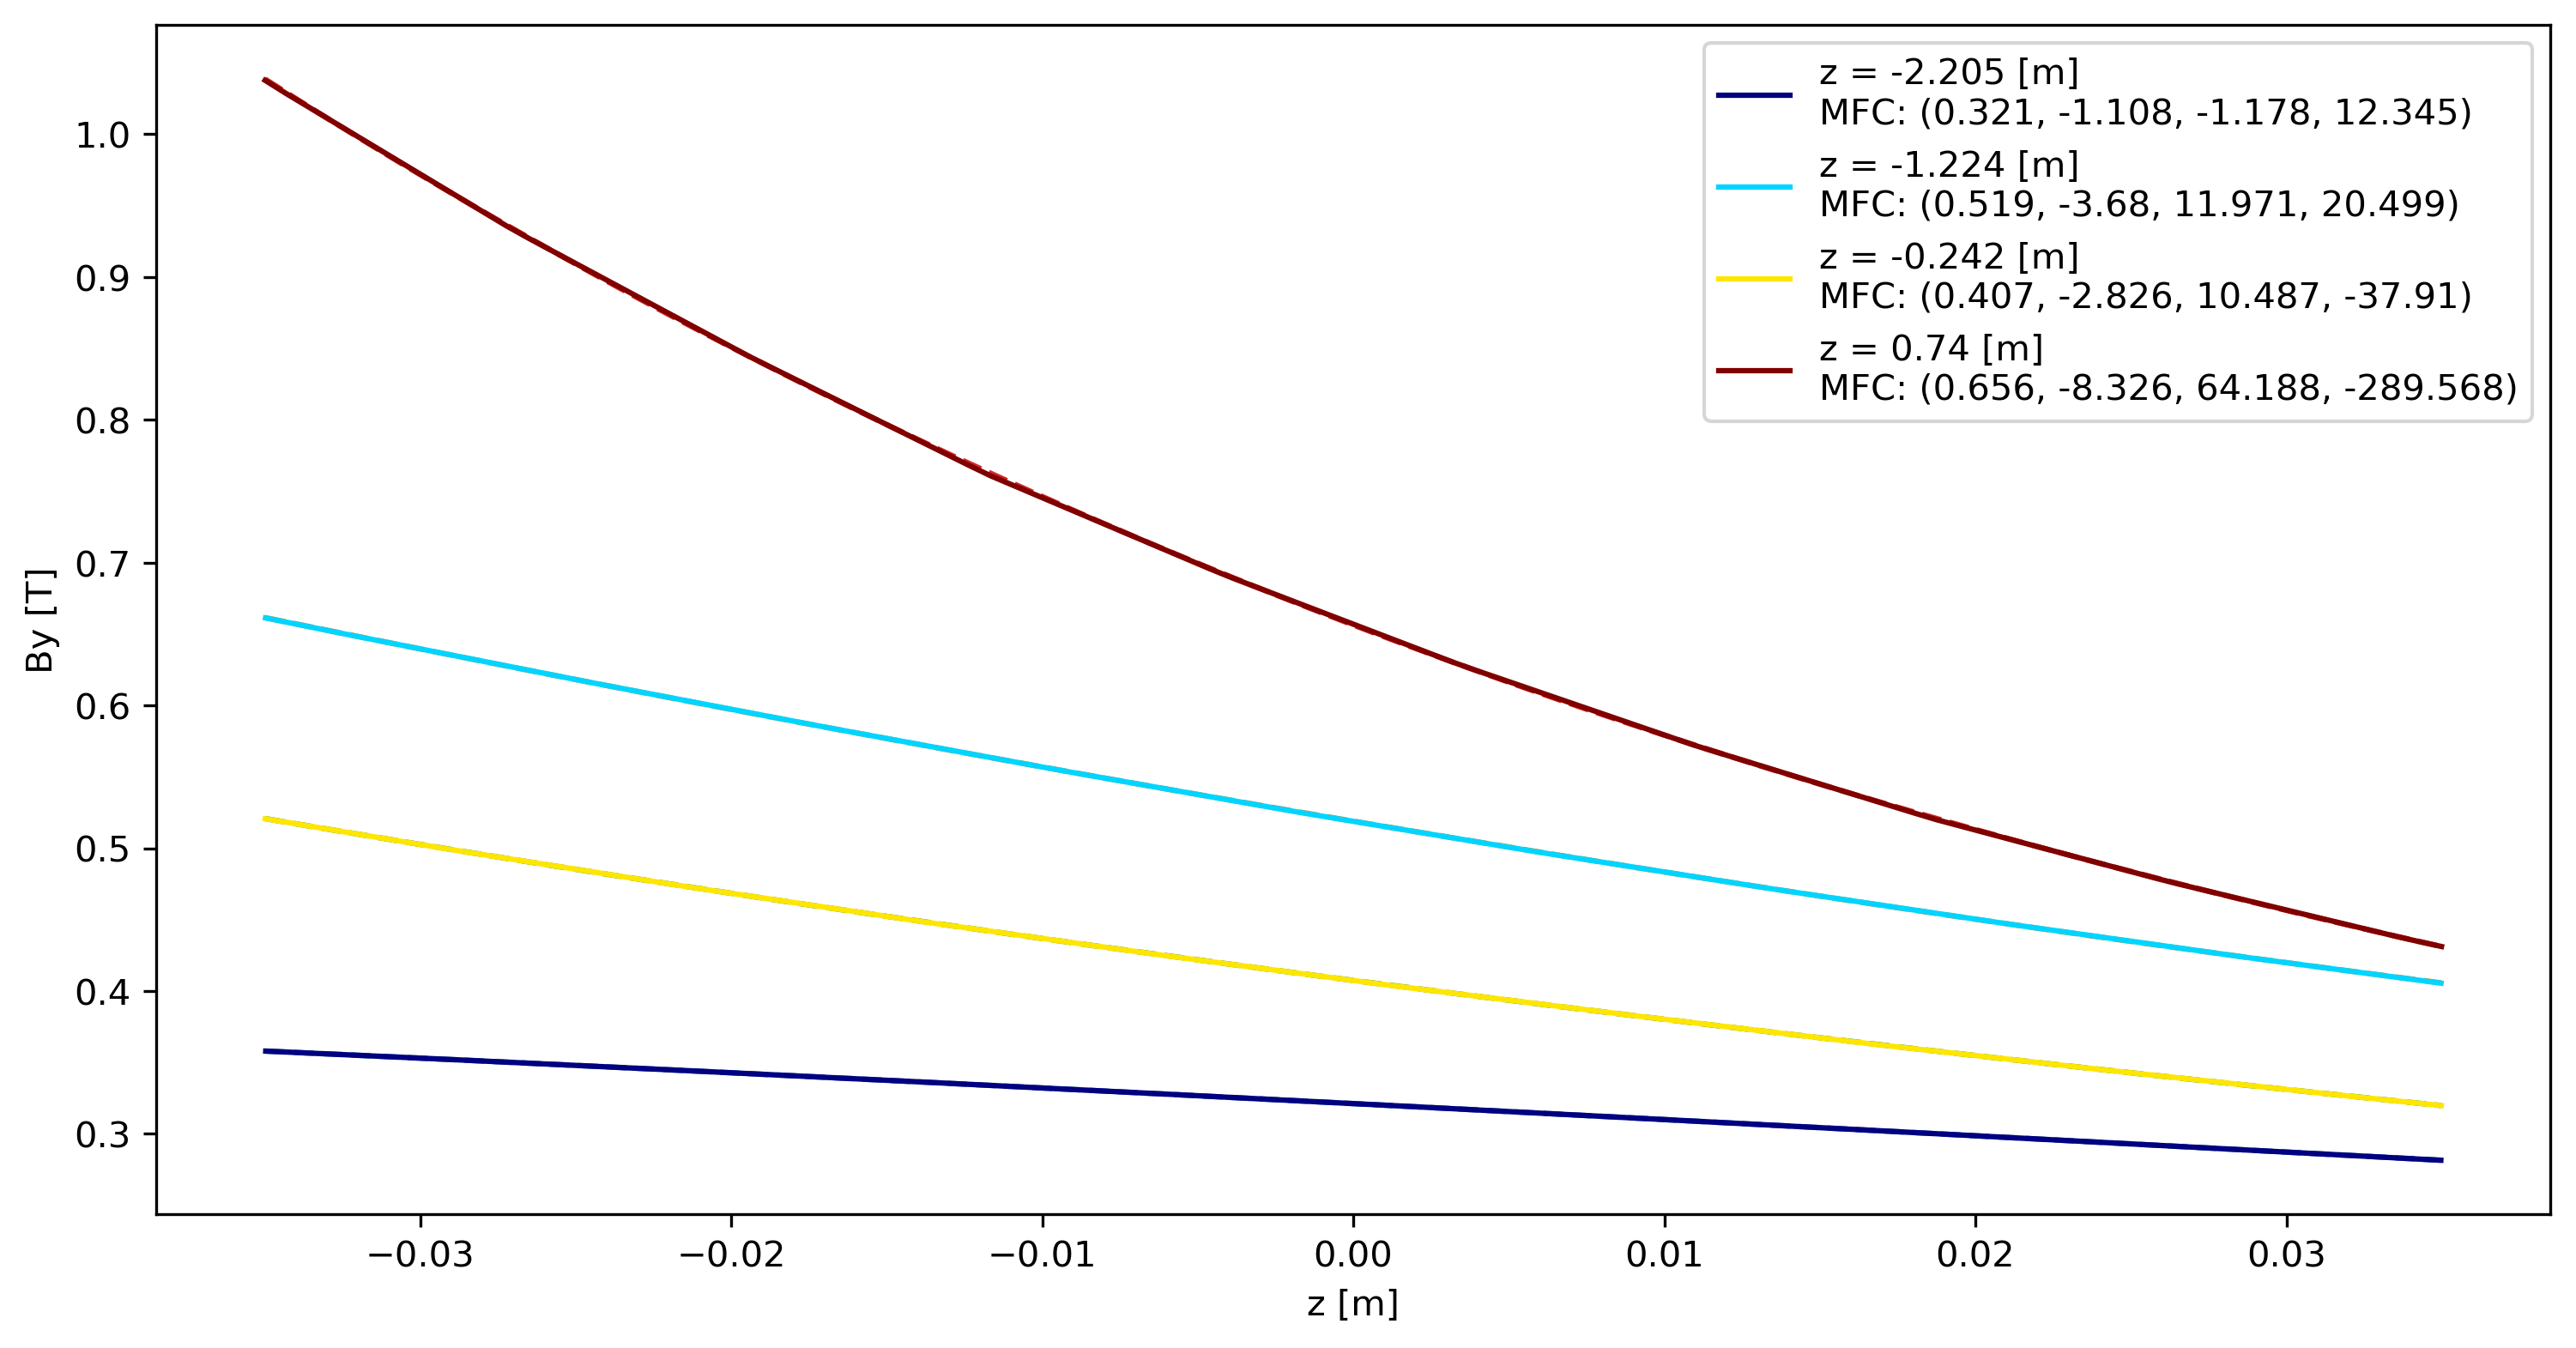
\includegraphics[width=0.7\textwidth]{02_Simulation/images/track_mu62_2_mfc.png}
\caption{Tracking of the proton beam in MU62 MFC transverse dipoles component.\textcolor{red}{The x-label should be $x_{T}$} }
\label{fig:track_mu62_2_mfc}
\end{figure}

Full tracking with along the beam line gives us the following MFC shown.

\begin{figure}[H]
\centering
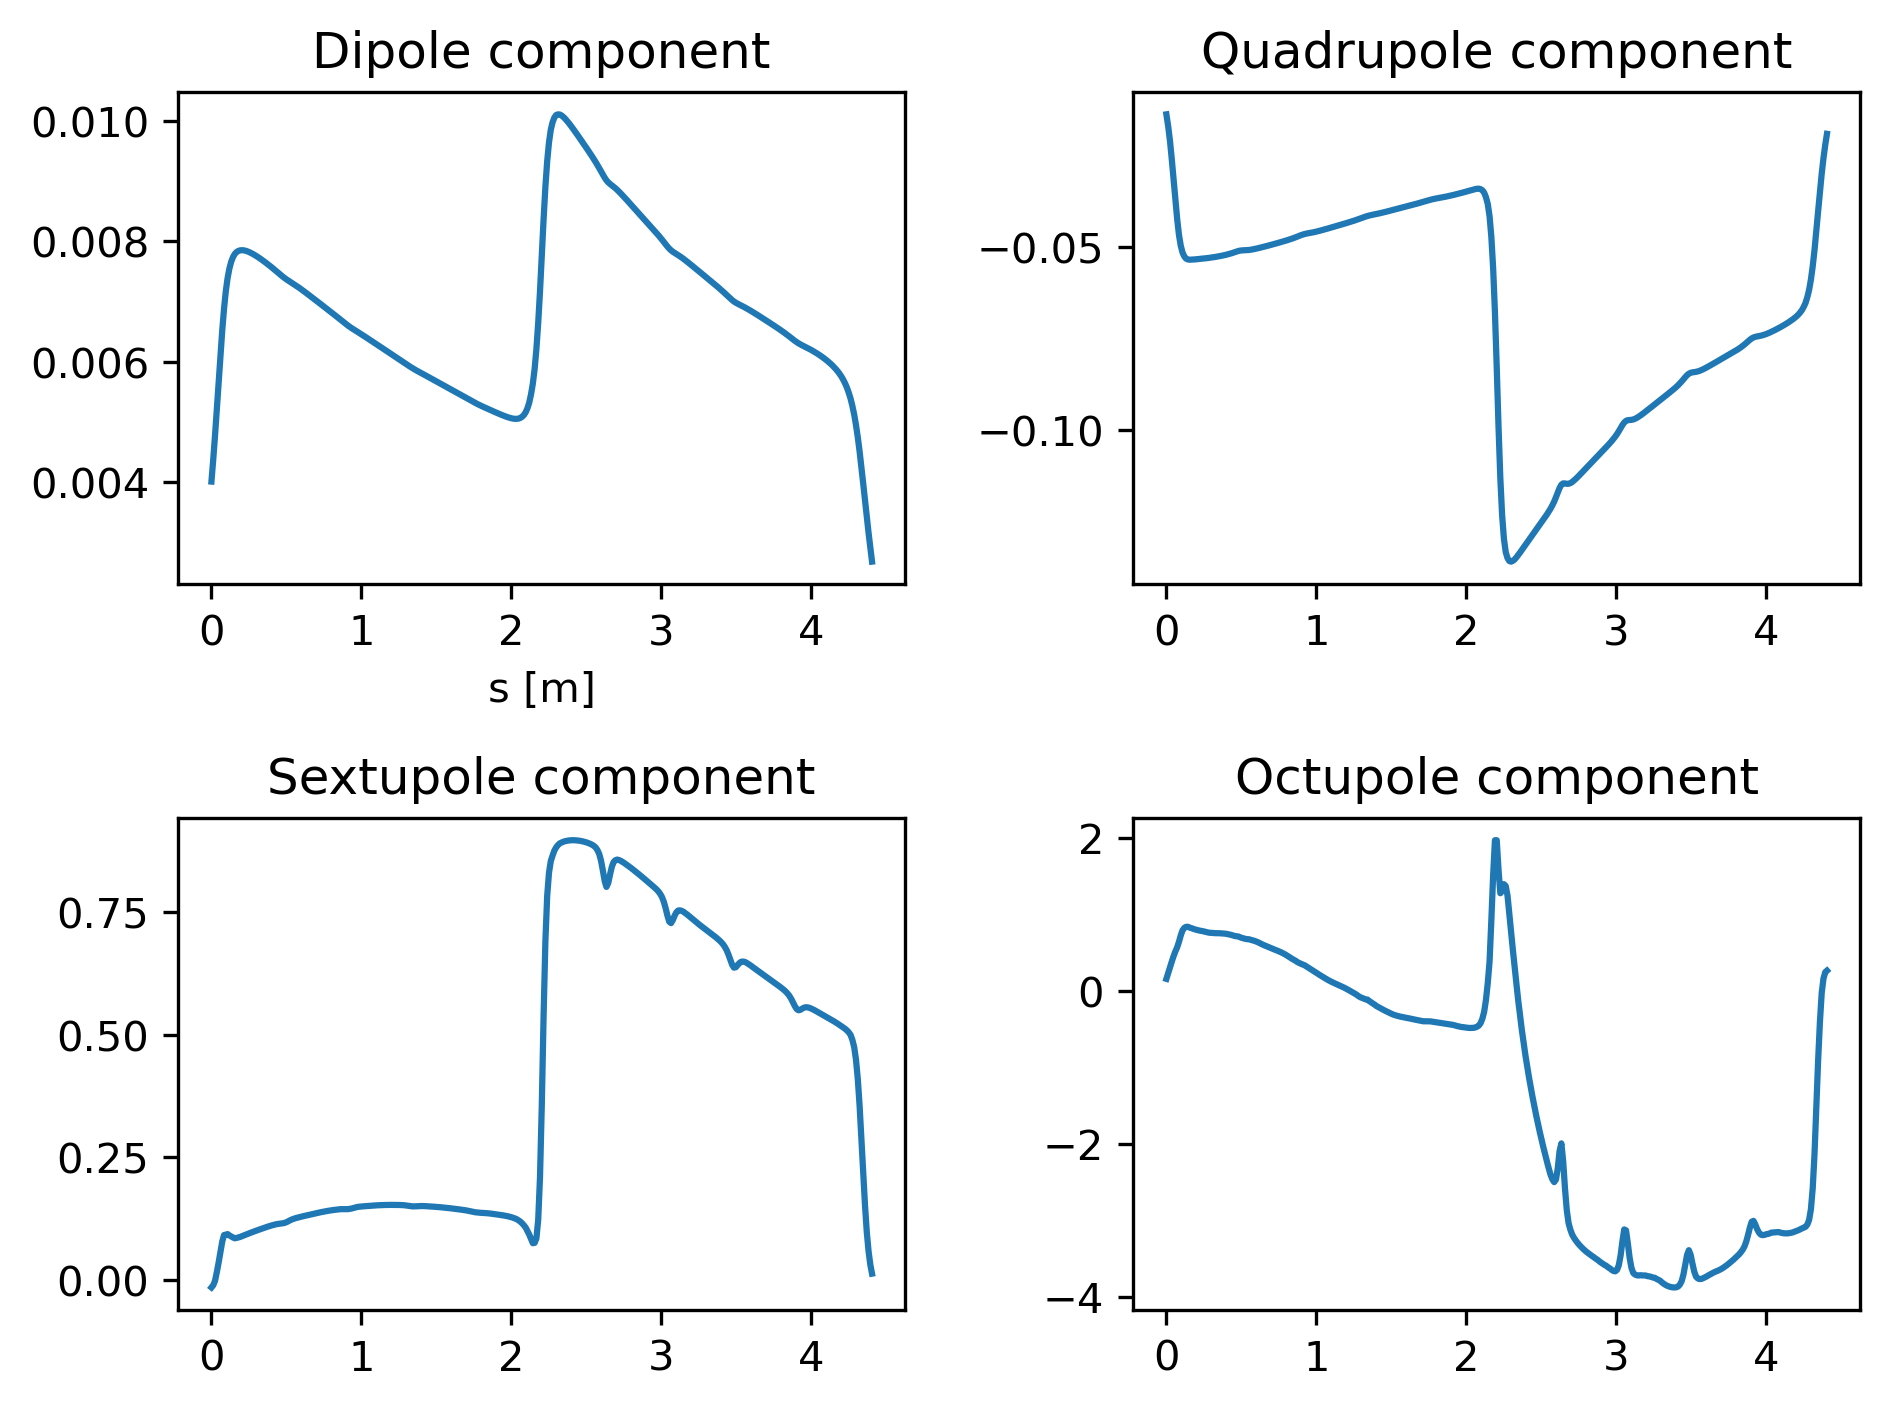
\includegraphics[width=0.7\textwidth]{02_Simulation/images/mfc_mu62.png}
\caption{MFC in MU62.}
\label{fig:mfc_mu62}
\end{figure}

Theses MFC components can be exported to a file to be used in MAD-X. The format for the \texttt{.ele} file is as follows:

\begin{lstlisting}
stray1 : multipole, knl:={2.11E-07,-3.11E-06,5.25E-05,-0.001056026};
stray2 : multipole, knl:={2.78E-07,-4.03E-06,6.74E-05,-0.001303161};
stray3 : multipole, knl:={3.54E-07,-5.09E-06,8.47E-05,-0.001548501};
\end{lstlisting}

When you export the multipole component you need to multiply by the length of the multipole element i.e.:

\[
\frac{L_{\text{Total}}}{l_{\text{element}}}
\]

The format for the \texttt{.seq} file is as follows:

\begin{lstlisting}
stray1, at = 29.9366067;
stray2, at = 29.9566067;
stray3, at = 29.9766067;
\end{lstlisting}

\subsection{Initial condition in F61D}

The MFC model was added to the F61D transfer line in MAD-X, see Fig. \ref{fig:f61d_with_stray}. The F61D with stray field line \href{https://gitlab.cern.ch/eljohnso/acc-models-tls-eliott-fork/-/blob/c6cbcafacca274000d2bfc501f39cf711375de90/ps_extraction/east-fast-extraction/f61d_with_stray/F61D_with_stray.ipynb}{script} has the stray field element of the MU62 magnet decomposed into multipole and can be found at \href{https://gitlab.cern.ch/eljohnso/acc-models-tls-eliott-fork/-/blob/c6cbcafacca274000d2bfc501f39cf711375de90/ps_extraction/east-fast-extraction/f61d_with_stray/strayMU62.ele}{strayMU62.ele} and \href{https://gitlab.cern.ch/eljohnso/acc-models-tls-eliott-fork/-/blob/c6cbcafacca274000d2bfc501f39cf711375de90/ps_extraction/east-fast-extraction/f61d_with_stray/strayMU62.seq}{strayMU62.seq}.

\begin{figure}[H]
\centering
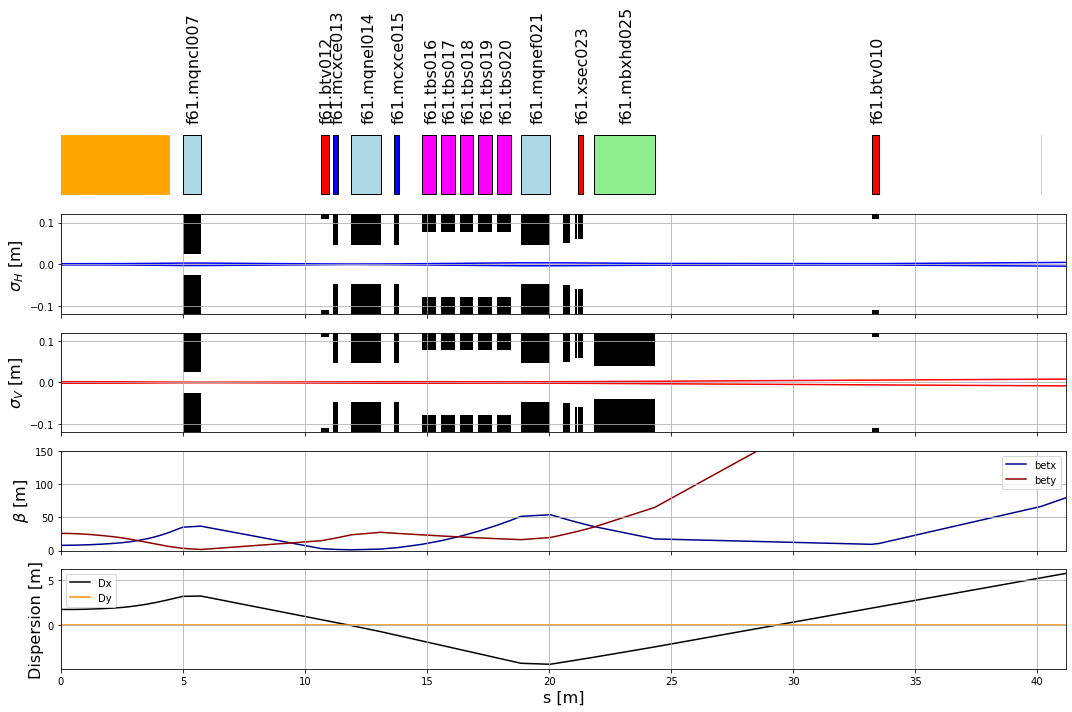
\includegraphics[width=1.0\textwidth]{02_Simulation/images/F61D_with_stray.png}
\caption{F61D with stray field multipole of MU62. The orange rectangle in the synoptic represents the multipole component of the stray field.}
\label{fig:f61d_with_stray}
\end{figure}


The initial condition of the F61D transfer line were found using the twiss parameters from the PS Ring slow extraction \href{https://gitlab.cern.ch/eljohnso/acc-models-tls-eliott-fork/-/blob/EliottBranch/ps_extraction/east-fast-extraction/Check%20scripts/slow_extraction_trajectory_maptrack_inital_conditions.ipynb}{script}. The beam enveloppe was extracted using a pycollimate simulation and retrieving the four particles marking the edge of the extracted separatrix, see Fig. \ref{fig:init_pycollimate}. The tune of the PS was match to be on resonance and the chromaticity match to measurement from 12.11.2021 (Qxp=-1.239, Qyp=0.242). These four particles were tracked during their last turn before being extracted in the PS with the electrostatic septum and the magnetic septa on. The strength of the electrostatic septum (SEH23) was determined by applying a voltage of \SI{-177}{\kilo\volt} across a gap of \SI{15.11}{\milli\metre}, resulting in an electric field of \SI{11.708}{\mega\volt\per\metre}. Given an effective length of \SI{0.8}{\metre}, the resulting strength was calculated as $\theta_{SEH23} = \arctan \left( \frac{|\mathbf{E}| \cdot \text{effective length}}{p \cdot \beta \cdot 10^9} \right)$, and incorporated into the MAD-X input as $kPESEH23$.

For the magnetic septa, the strength of SMH57 was derived from a current of \SI{9120}{\ampere} (measured on 12.11.21), scaled from codilog data to obtain a strength of $\theta_{SMH57} = \frac{\text{current} \cdot 0.378}{9871 \cdot \mathbf{B} \rho}$, which was input into MAD-X as $kPESMH57$. Similarly, SMH61 had a measured current of \SI{1170}{\ampere} (measured on 12.11.21), with a strength calculated as $\theta_{SMH61} = \frac{\text{current} \cdot 0.247}{2350 \cdot \mathbf{B} \rho}$, and input into MAD-X as $kPESMH61$.



\begin{figure}[H]
\centering
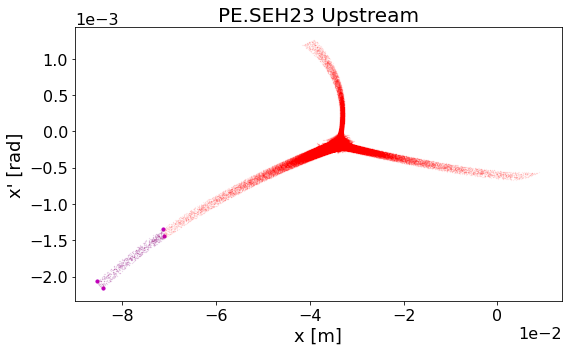
\includegraphics[width=0.7\textwidth]{02_Simulation/images/init_pycollimate.png}
\caption{Distribution of particles in the PS and the four particles at the extremity of the separatrix used as beam envelope.}
\label{fig:init_pycollimate}
\end{figure}

Figure \ref{fig:beam_envelope} shows the envelope of the slow extraced beam from the PS to the East Area. This simulation was used to calculate the initial conditions before entering the stray fields of MU62.


\begin{figure}[H]
\centering
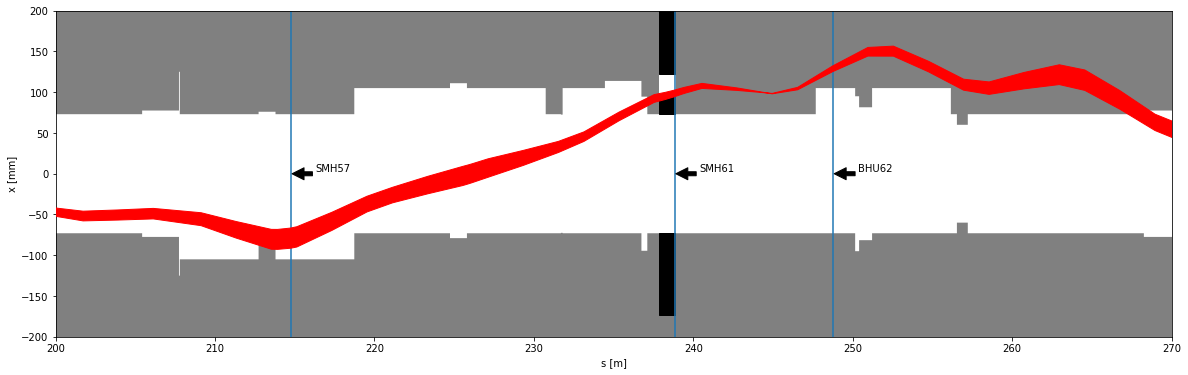
\includegraphics[width=1.0\textwidth]{02_Simulation/images/beam_envelope.png}
\caption{Beam envelope through SMH57, SMH61 and at the entrance of MU62.}
\label{fig:beam_envelope}
\end{figure}

\begin{table}[ht]
    \centering
    \caption{Initial condition upstream of the MU62 magnet}
    \begin{tabular}{l c}
        \hline
        \textbf{Twiss Parameter} & \textbf{Value} \\
        \hline
        $\beta_{x0}$ & 7.48 \\
        $\beta_{y0}$ & 26.14 \\
        $\alpha_{x0}$ & 0.0021 \\
        $\alpha_{y0}$ & 0.0591 \\
        $D_{x0}$ & 1.428 \\
        $D_{y0}$ & 0.0 \\
        $D'_{x0}$ & -0.021 \\
        $D'_{y0}$ & 0.0 \\
        \hline
    \end{tabular}
    \label{tab:twiss_parameters}
\end{table}

\begin{table}[ht]
    \centering
    \caption{Comparison of Simulated and Measured Twiss Parameters after the MU62 stray fields.}
    \begin{tabular}{l c c}
        \hline
        \textbf{Twiss Parameter} & \textbf{Simulated} & \textbf{Measured} \\
        \hline
        $\beta_{x0}$ & 35 & 154 \\
        $\beta_{y0}$ & 3.4 & 5.2 \\
        $\alpha_{x0}$ & -7.4 & -37 \\
        $\alpha_{y0}$ & 2.1 & 0.25 \\
        $D_{x0}$ & 3.2 & 0.13 \\
        $D_{y0}$ & 0 & 0 \\
        $D'_{x0}$ & 0.63 & 0.02 \\
        $D'_{y0}$ & 0 & 0 \\
        \hline
    \end{tabular}
    \label{tab:twiss_comparison}
\end{table}

The comparison of the simulated and measured Twiss parameters after the MU62 stray fields reveals significant discrepancies. The simulated values for $\beta_{x0}$, $\alpha_{x0}$, and $D_{x0}$ show considerable deviations from the measured data, with the simulated $\beta_{x0}$ and $\alpha_{x0}$ being notably lower than the measured values. These differences suggest that the simulation model does not accurately capture the conditions observed in the empirical measurements. Further investigation is required to identify the underlying causes of these discrepancies and to improve the accuracy of the simulation model. Adjustments to the model parameters or the inclusion of additional physical effects might be necessary to achieve better alignment between simulation and measurement.

\subsection{Stitched model}

The slow extraction cannot be transported with a twiss, you need to perform tracking. The distribution on the edge of the septum blade make three turns and are extracted on the fourth one, whereas the ones outside the septum blade are extracted in the present turn.

The \href{https://gitlab.cern.ch/eljohnso/acc-models-tls-eliott-fork/-/blob/EliottBranch/ps_extraction/east-fast-extraction/stitched_slow_extraction_east_PTC_single_turn.ipynb}{script} tracks the pycollimate distribution in the PS, save the distribution at the entrance of MU62, remove the mean x and xp and then tracks it in the F61D line. This simulation also include the MFC of MU63.


\begin{table}[ht]
    \centering
    \caption{Twiss Parameters from Distribution}
    \begin{tabular}{l c}
        \hline
        \textbf{Twiss Parameter} & \textbf{Value} \\
        \hline
        $\beta_x$ & 167.32 \\
        $\alpha_x$ & 21.61 \\
        $\beta_y$ & 1.21 \\
        $\alpha_y$ & 0.33 \\
        $\epsilon_x$ & $1.78 \times 10^{-7}$ \\
        $\epsilon_y$ & $3.8 \times 10^{-8}$\\
        \hline
    \end{tabular}
    \label{tab:twiss_distribution}
\end{table}


\begin{figure}[H]
\centering
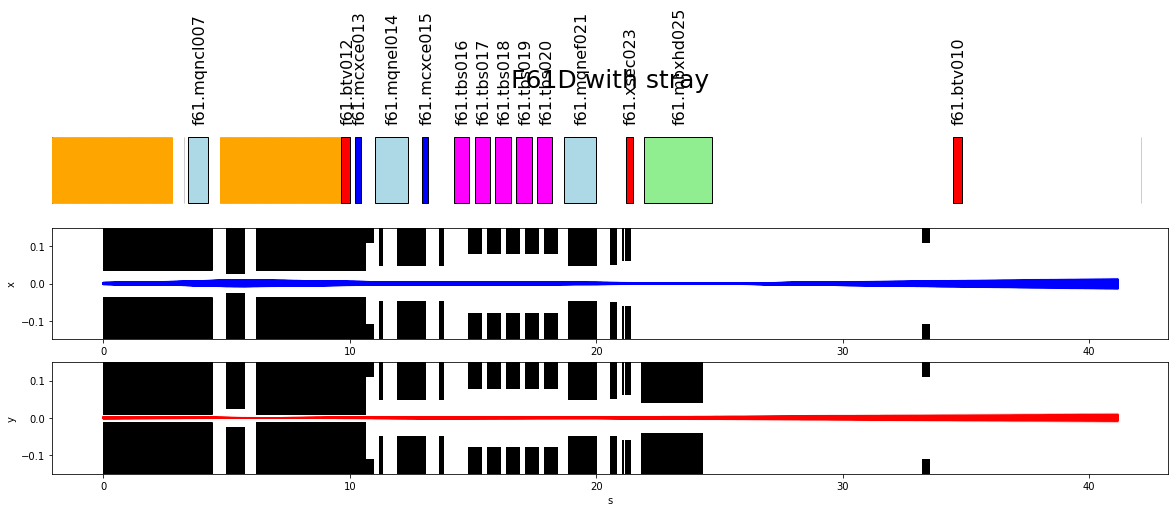
\includegraphics[width=1.0\textwidth]{02_Simulation/images/PTC_stray_field.png}
\caption{Stitched model PTC tracking.}
\label{fig:stitched_PTC}
\end{figure}

\subsection{Repository with the Full Stitching fomr the PS Ring to the East Dump}

The repository name is \href{https://gitlab.cern.ch/eljohnso/stray-fields}{stray-fields}. 

Step one, you need to create the distribution upstream of SEH23 using pycollimate. This is done in this \href{https://gitlab.cern.ch/eljohnso/stray-fields/-/blob/master/pycollimate.ipynb}{script} which gives you the distribution\_at\_seh23.pkl file.

Step two is to run \href{https://gitlab.cern.ch/eljohnso/stray-fields/-/blob/master/ps_ring.ipynb?ref_type=heads}{ps ring} which tracks the particle distribution in the PS ring and outputs the distribution before entering in the MU62

Step three is to run \href{https://gitlab.cern.ch/eljohnso/stray-fields/-/blob/master/f61d_tracking.ipynb?ref_type=heads}{f61d tracking} which takes the distribution entering in MU62 and tracking it in the F61D line.

\begin{figure}[H]
\centering
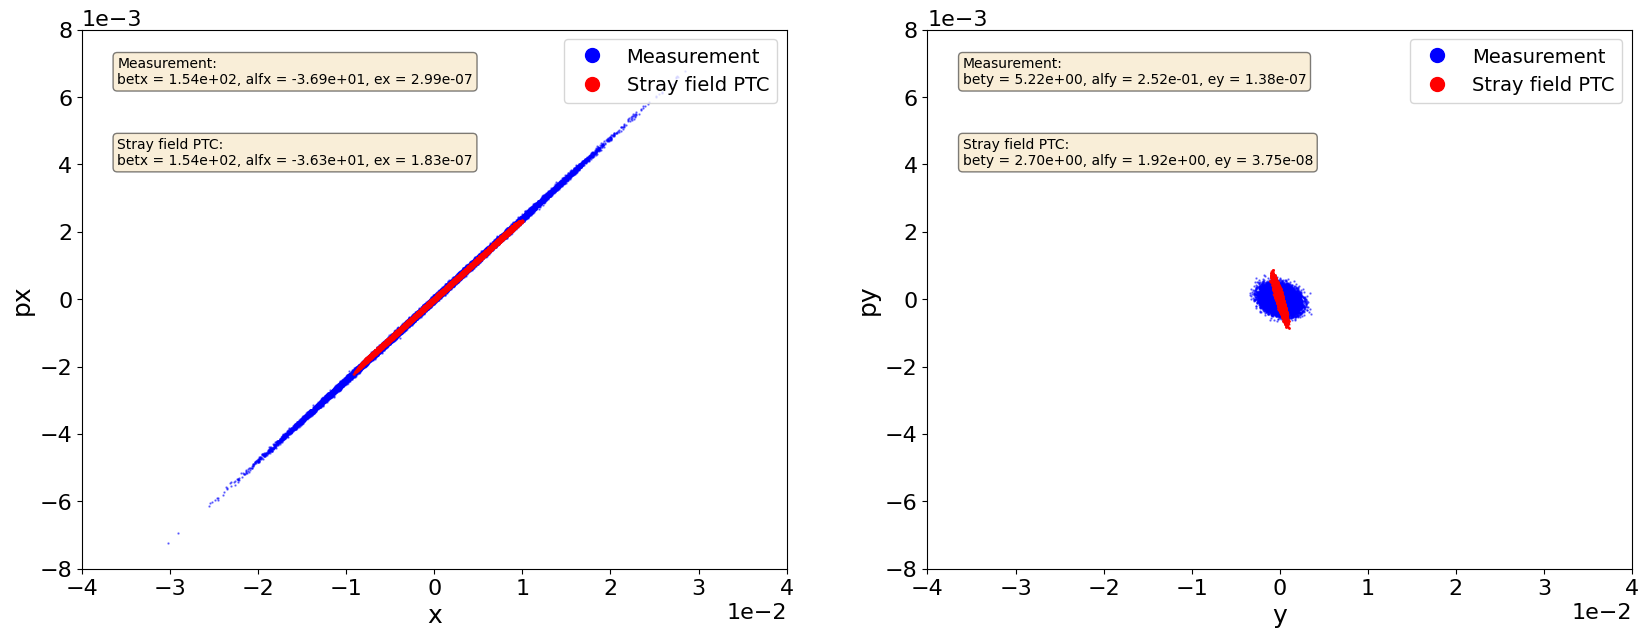
\includegraphics[width=1.0\textwidth]{02_Simulation/images/full_stitching_PTC.png}
\caption{Full Stitched model PTC tracking.}
\label{fig:full_stitched_PTC}
\end{figure}

Something to note is that the distribution from tracking is non gaussian so when computing the twiss parameters there might be some discrepancy.

\begin{figure}[H]
\centering
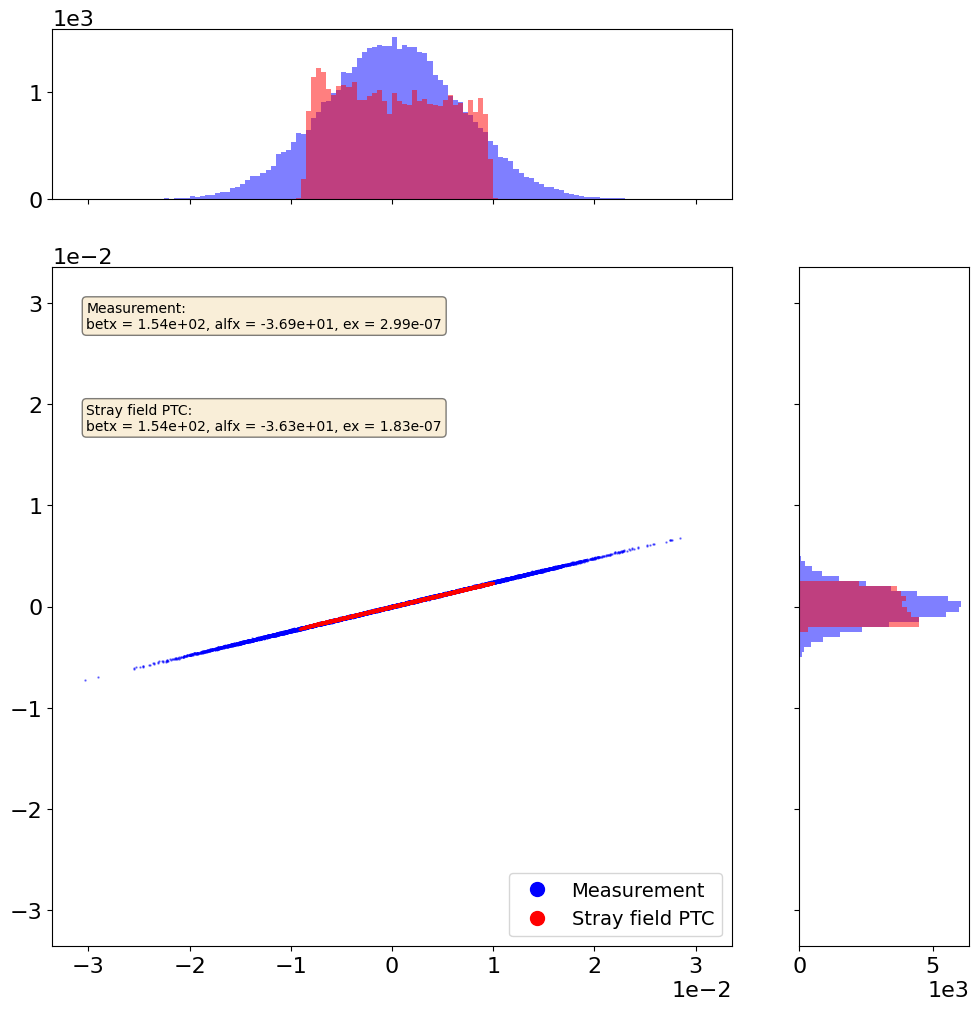
\includegraphics[width=1.0\textwidth]{02_Simulation/images/non_gaussian.png}
\caption{The distributions are not gaussian.}
\label{fig:full_stitched_PTC}
\end{figure}

Perhaps instead of showing distribution of particles it is interesting to see the difference in the ellipses, see Fig. \ref{fig:ellipses.}.

\begin{figure}[H]
\centering
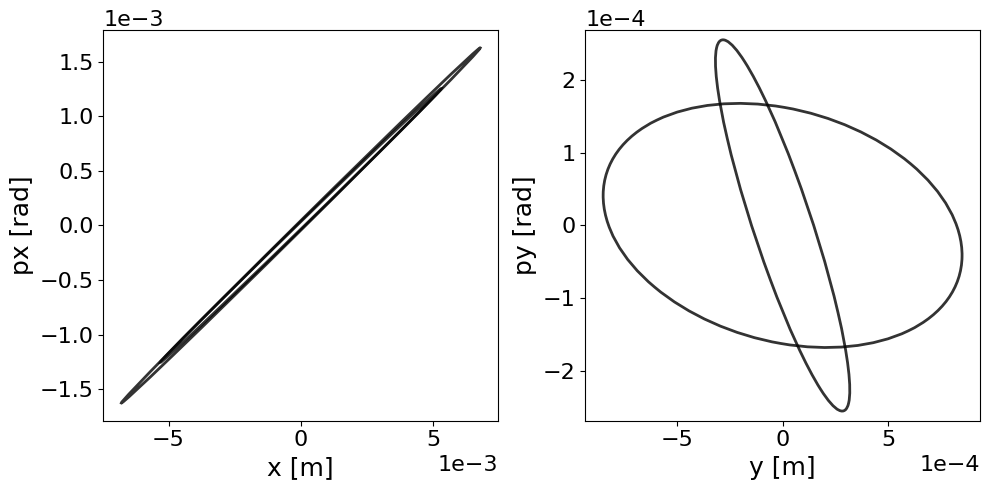
\includegraphics[width=1.0\textwidth]{02_Simulation/images/ellipses.png}
\caption{Comparison between the ellipses produces by the twiss parameters of the simulation and the tracking.}
\label{fig:ellipses.}
\end{figure}

We can also have a look at the twiss parameters evolution along the line, see Fig. \ref{fig:twiss_params}.

\begin{figure}[H]
\centering
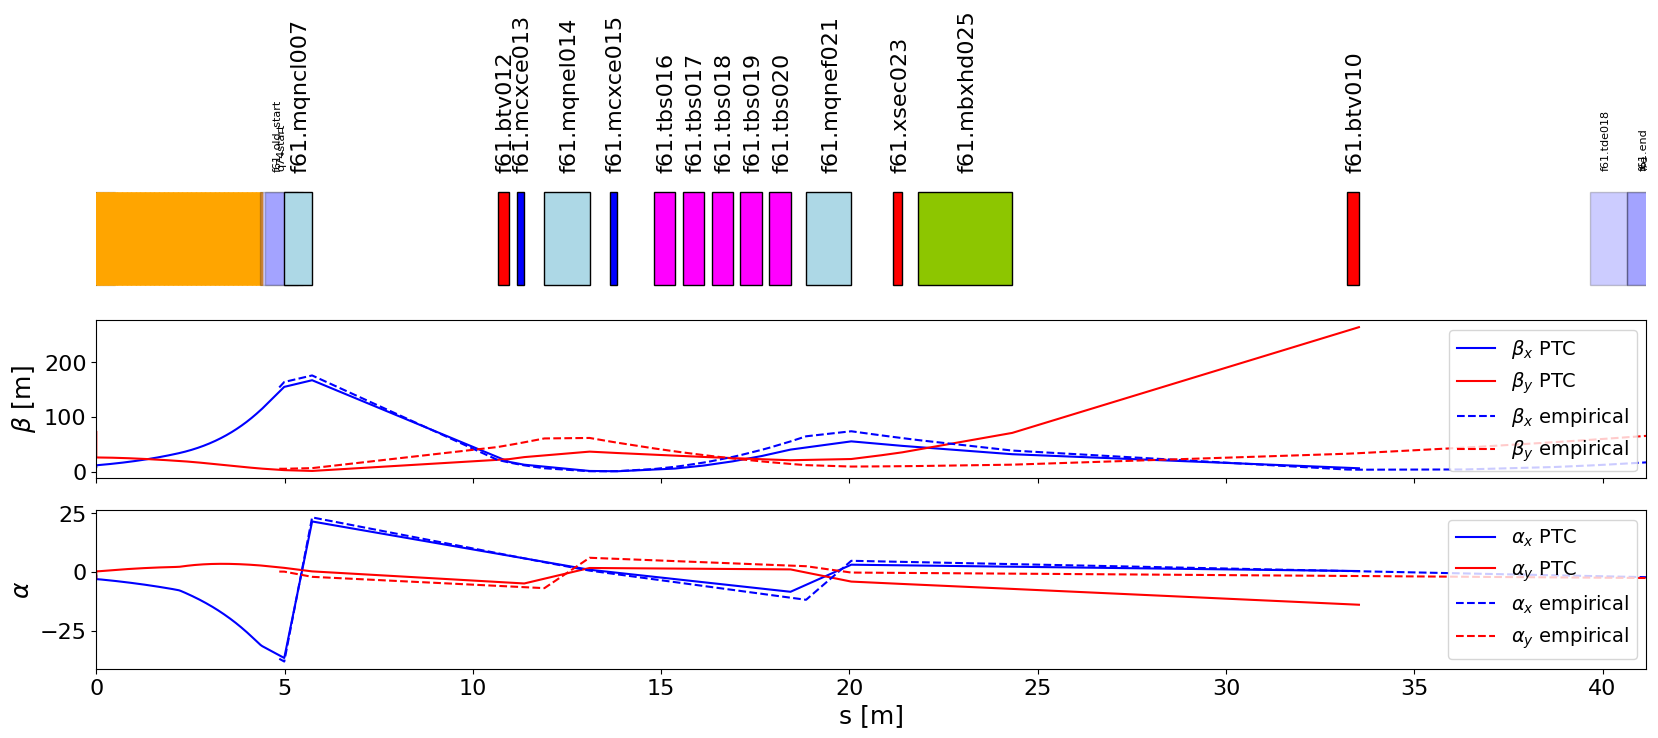
\includegraphics[width=1.0\textwidth]{02_Simulation/images/twiss_parameters_comparison.png}
\caption{Comparison between the twiss parameters along the line of the simulation and the tracking.}
\label{fig:twiss_params}
\end{figure}

\subsection{Simulation of Transfer Matrix Using Tracking at Injection}

The following subsection describes the methodology and findings from a simulation study aimed at constructing a transfer matrix for the injection process in the Proton Synchrotron (PS) using tracking techniques. The primary objective is to evaluate the response of injected particles to various initial offsets and to compare the results with existing models.

A comprehensive simulation was performed using the  \href{https://gitlab.cern.ch/eljohnso/acc-models-tls-eliott-fork/-/blob/EliottBranch/ps_injection/kick_response_injection_tracking/kick_response_BTP_injection_loop_transfer_matrix.ipynb}{kick response BTP injection loop transfer matrix} notebook. This notebook tracks particles injected into the PS at different initial offsets in the transverse and longitudinal planes. Specifically, four types of initial offsets were used: horizontal position (\(x_{in}\)), horizontal angle (\(p_{x,in}\)), vertical position (\(y_{in}\)), and vertical angle (\(p_{y,in}\)). The resulting offsets at the output (\(x_{out}\), \(p_{x,out}\), \(y_{out}\), \(p_{y,out}\)) were recorded to construct the transfer matrix.

\begin{figure}[H]
\centering
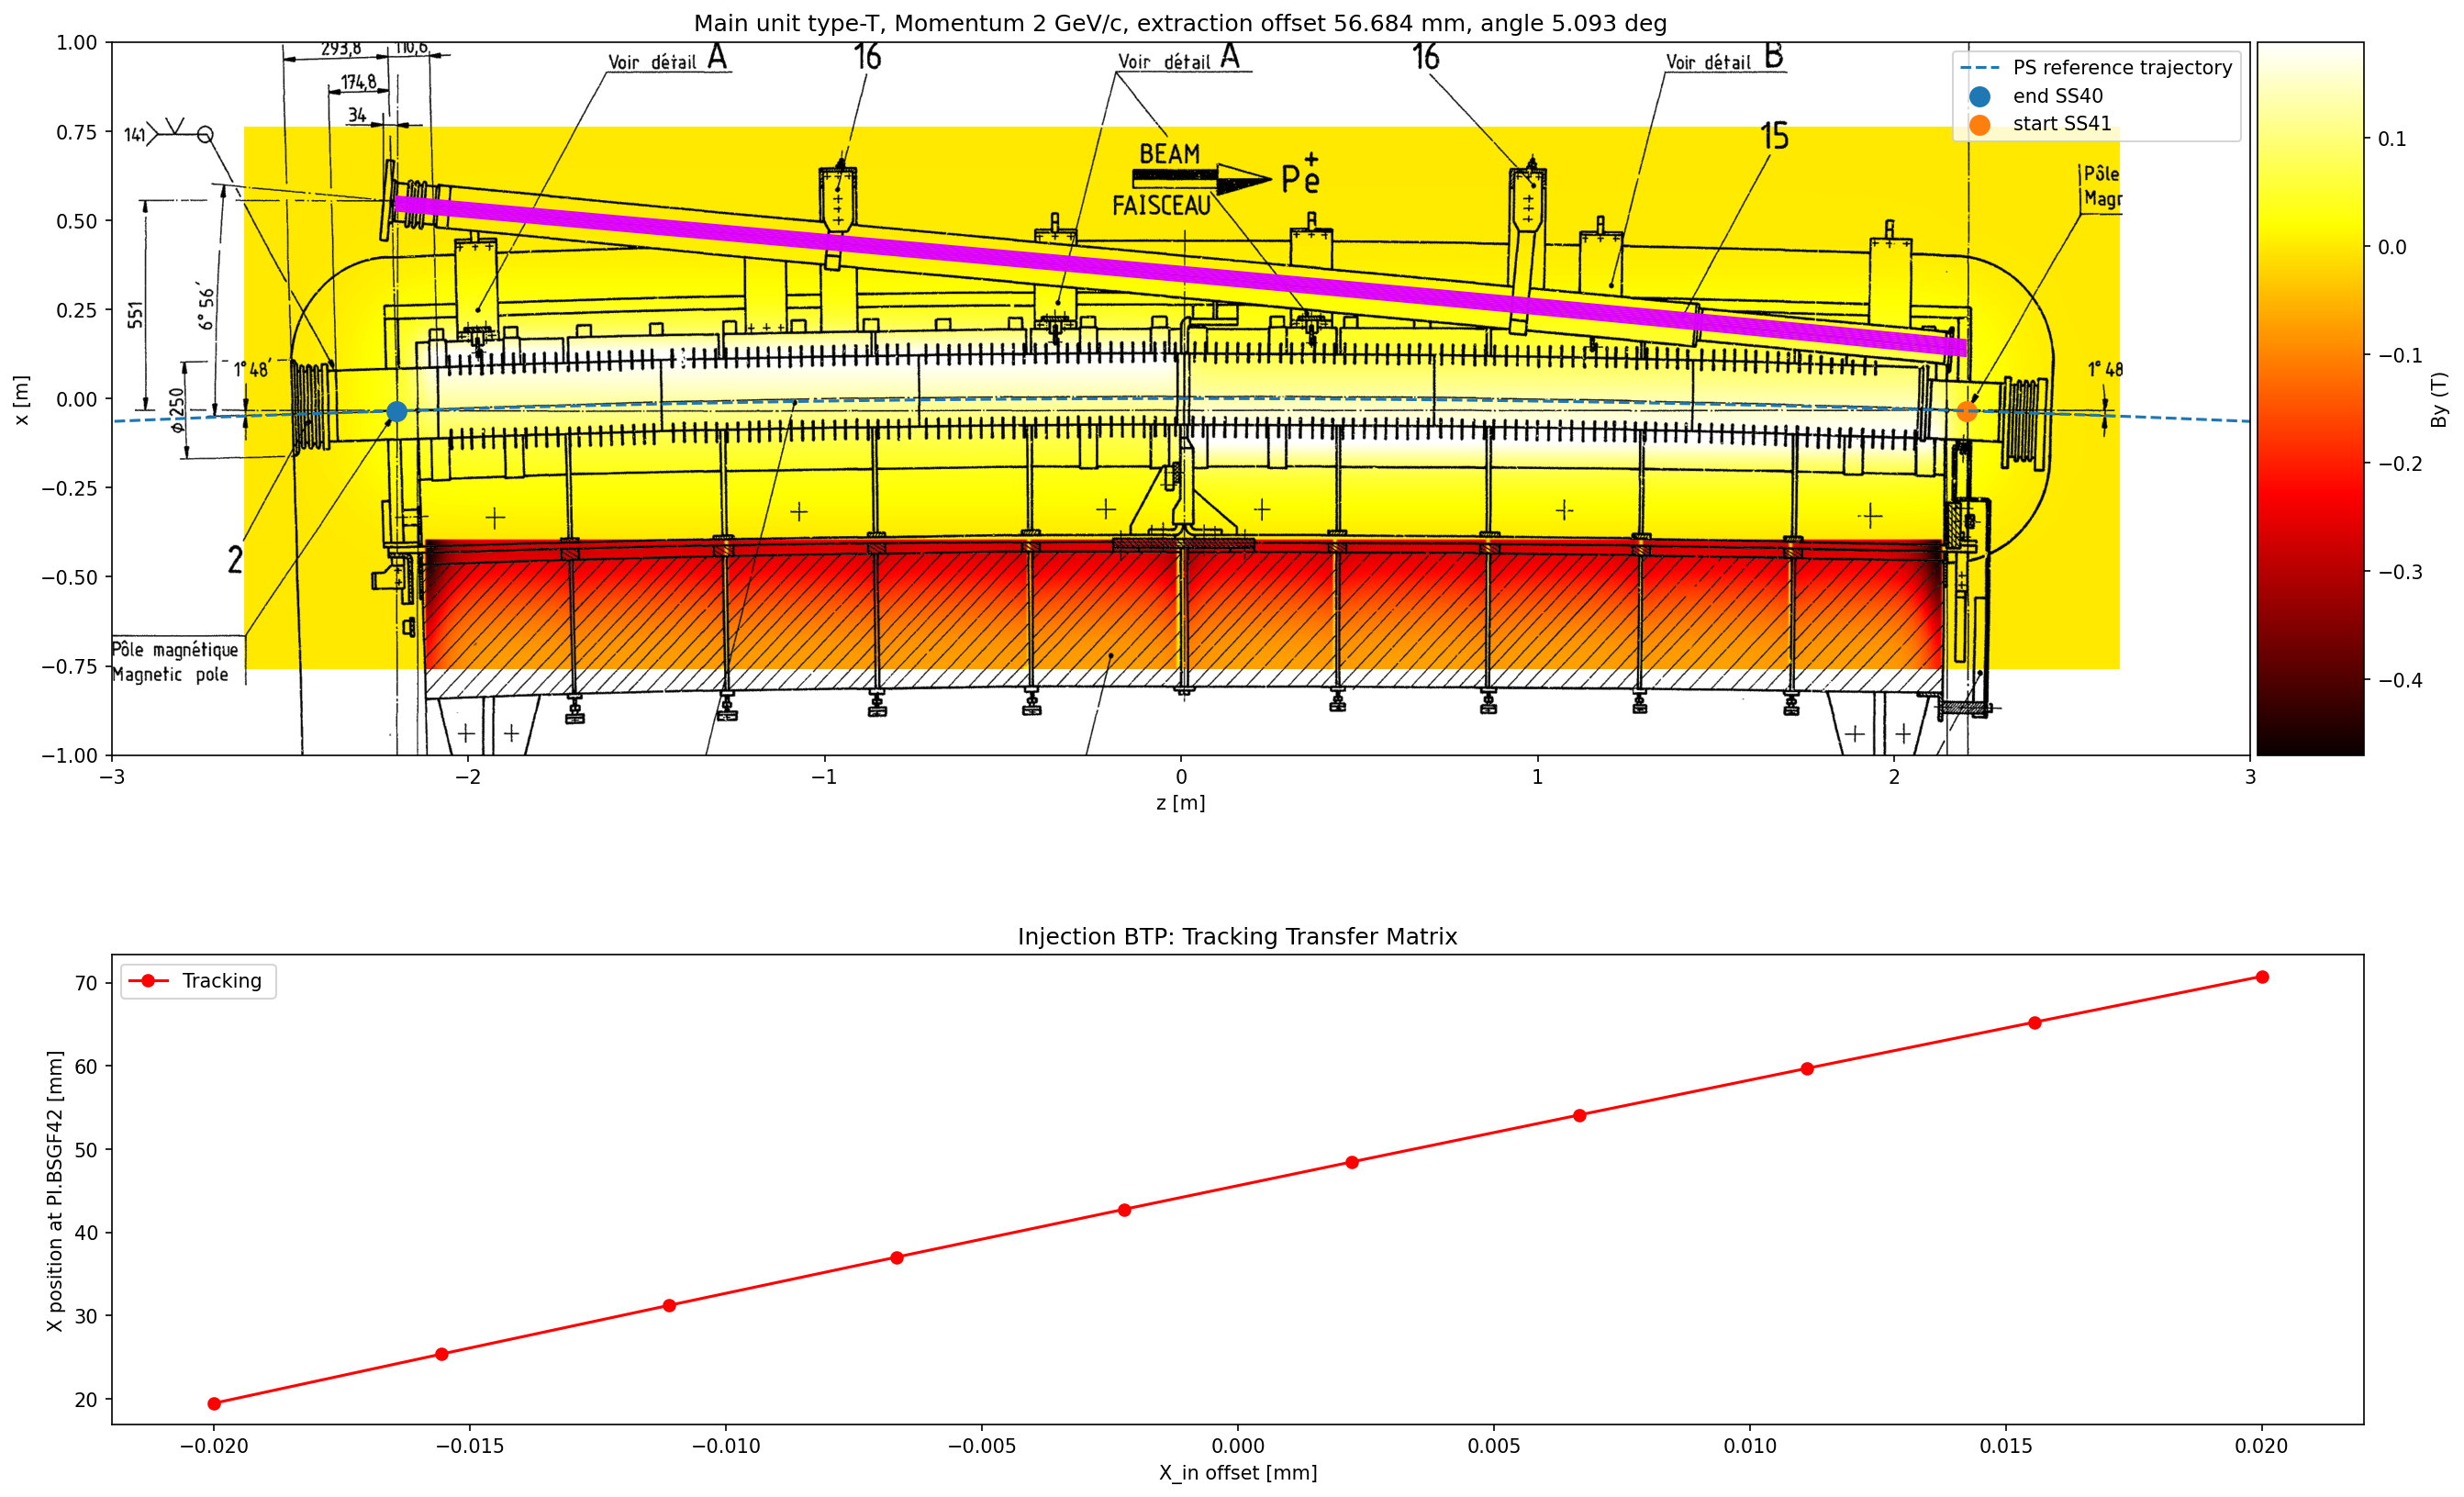
\includegraphics[width=1.0\textwidth]{02_Simulation/images/injection_transfer_matrix_1.png}
\caption{Building a transfer matrix through tracking.}
\label{fig:transfer_matrix_1}
\end{figure}

\begin{figure}[H]
\centering
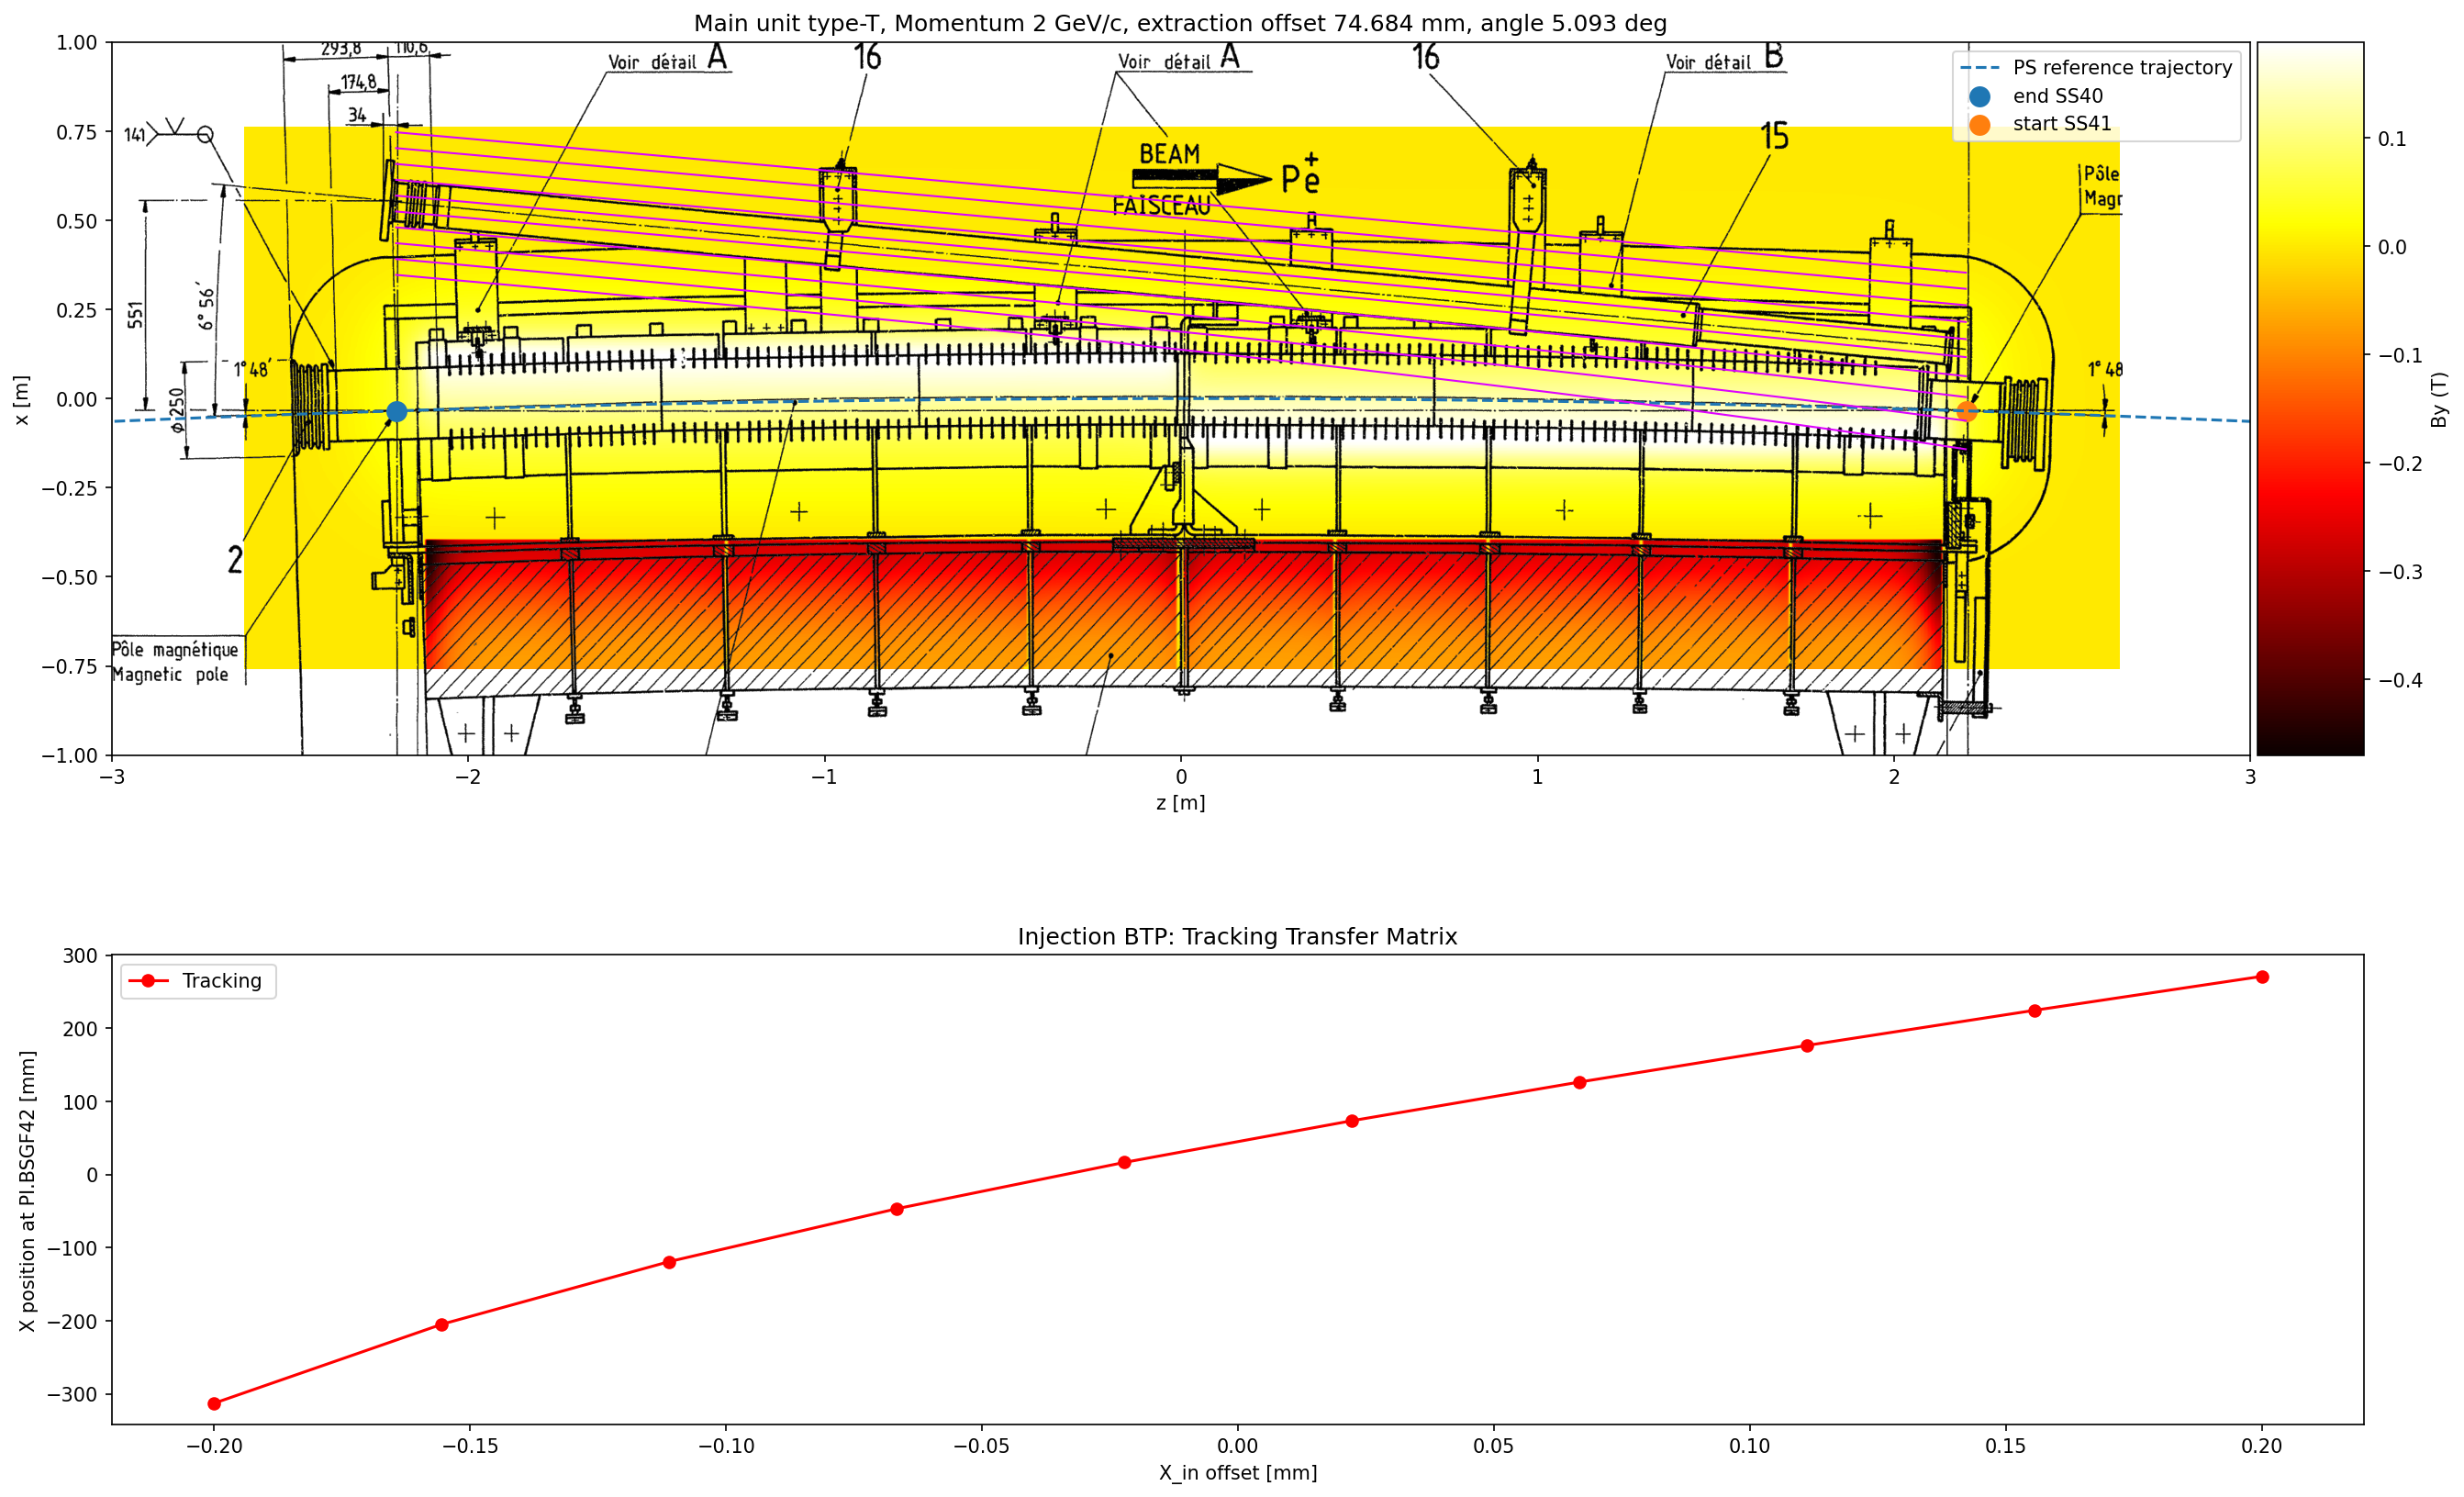
\includegraphics[width=1.0\textwidth]{02_Simulation/images/injection_transfer_matrix_2.png}
\caption{Wide scan of the position offset to see if the response is non-linear.}
\label{fig:transfer_matrix_2}
\end{figure}


The simulation can cover a wide range of offsets to capture potential non-linearities. The wide scan shown in Fig. \ref{fig:transfer_matrix_2} launches particles at transverse offsets that extend beyond the vacuum chamber, showing the non-linear beam dynamics.

As such, the technique to build a transfer matrix is to launch particles with four kind of input offsets: $x_{in}$, $xp_{in}$, $y_{in}$, $yp_{in}$ and record the output offsets $x_{out}$, $xp_{out}$, $y_{out}$, $yp_{out}$.

\begin{figure}[H]
\centering
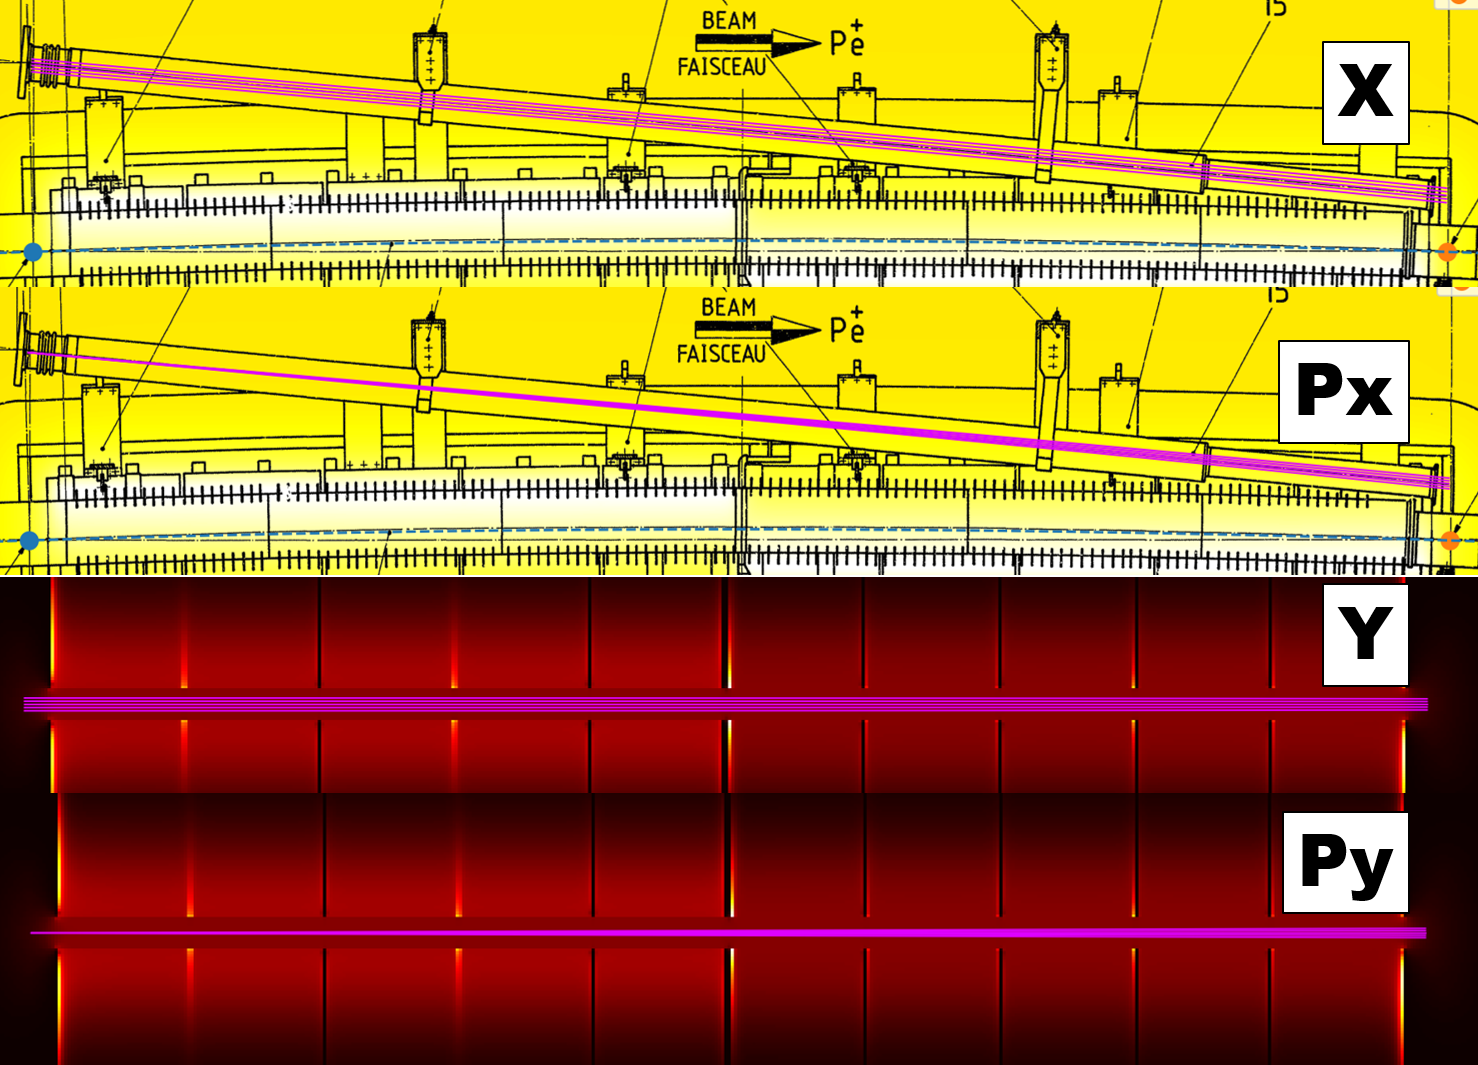
\includegraphics[width=1.0\textwidth]{02_Simulation/images/injection_transfer_matrix_3.png}
\caption{Particles are launched with different offsets.}
\label{fig:transfer_matrix_3}
\end{figure}

Figure \ref{fig:transfer_matrix_4} shows the transfer matrix points between the start and the end of the tracking inside the main unit. A linear fit is used to calculate the slope.

\begin{figure}[H]
\centering
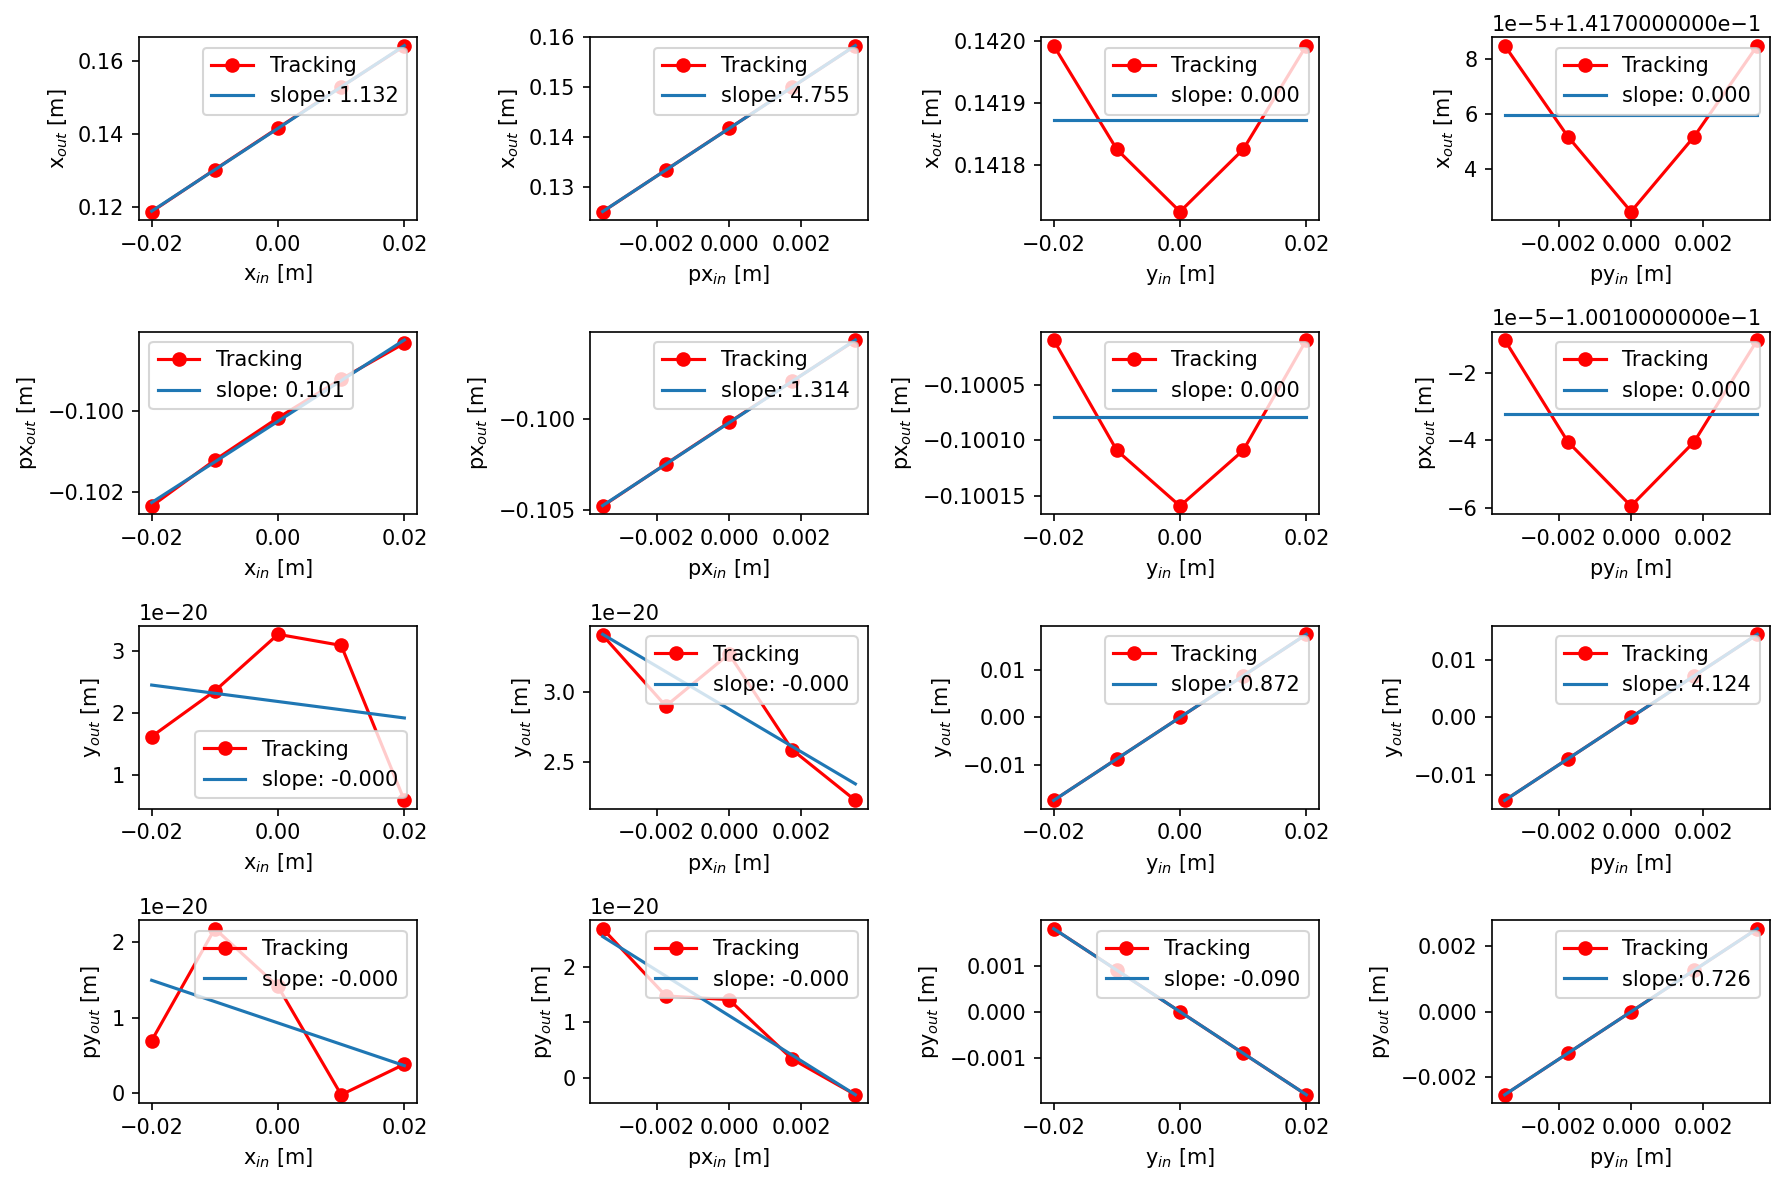
\includegraphics[width=1.0\textwidth]{02_Simulation/images/injection_transfer_matrix_4.png}
\caption{Particles are launched with different offsets.}
\label{fig:transfer_matrix_4}
\end{figure}



\textbf{Matrix from Tracking:}
\[
\begin{bmatrix}
1.132 & 4.755 & 0 & 0 \\
0.101 & 1.314 & 0 & 0 \\
0 & 0 & 0.872 & 4.124 \\
0 & 0 & -0.090 & 0.726
\end{bmatrix}
\]

The transfer matrix can also be visualized using color maps and compared to another transfer matrix tool developed by Ewa (called tracks.get\_transport\_matrix(k = k\_last, ret = 'mat')). Ewa's method eliminates the need for computationally intensive tracking. Instead, the nominal tracking can be used in conjunction with Ewa's function. However, it is important to note that this approach is only valid for the tracking section and does not extend to the SEM-Grid.

\begin{figure}[H]
\centering
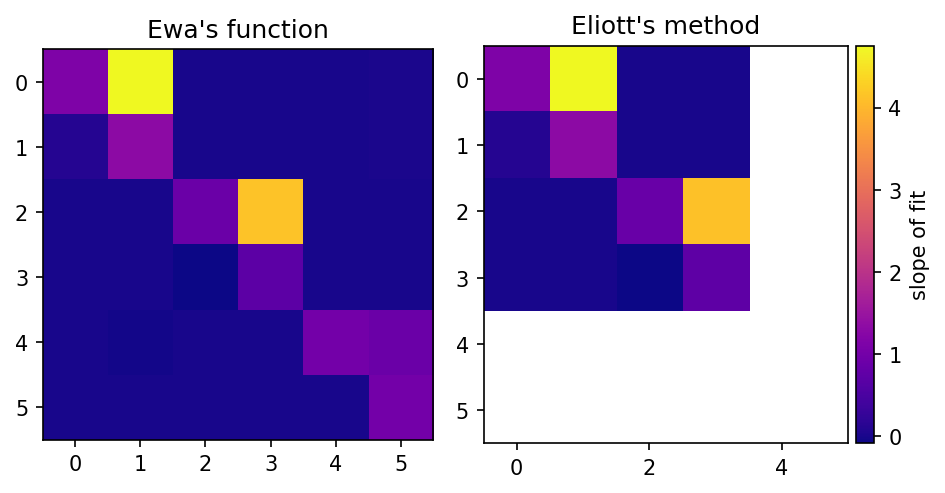
\includegraphics[width=1.0\textwidth]{02_Simulation/images/transfer_matrix_color.png}
\caption{Comparison between the matrix found by tracking at different offsets and Ewa's function.}
\label{fig:transfer_matrix_color}
\end{figure}





A transfer matrix, see Fig. \ref{fig:transfer_matrix_color}, can also be built as a function of POPS (from \si{500} to \si{1500}{gauss}) where it is observed that the injection angles are very sensitive to POPS change. The transfer matrix shows that injection angles are twice the sensitivity compared to horizontal (\(x\)) or vertical (\(y\)) offsets. This implies that any increase in POPS will significantly amplify the effect of a change in the horizontal angle (\(p_x\)) on the horizontal offset (\(x\)). Specifically, the matrix elements \(R_{21}\) and \(R_{22}\) exhibit the most substantial positive changes, indicating a strong correlation between \(p_{x,\text{in}}\) and both \(x_{\text{out}}\) and \(p_{x,\text{out}}\). Conversely, \(R_{34}\) and \(R_{44}\) show the most significant negative changes, highlighting the impact of \(p_{y,\text{in}}\) on both \(y_{\text{out}}\) and \(p_{y,\text{out}}\). These findings underscore the critical influence of POPS variations on beam dynamics, particularly in relation to injection angles.

\begin{figure}[H]
\centering
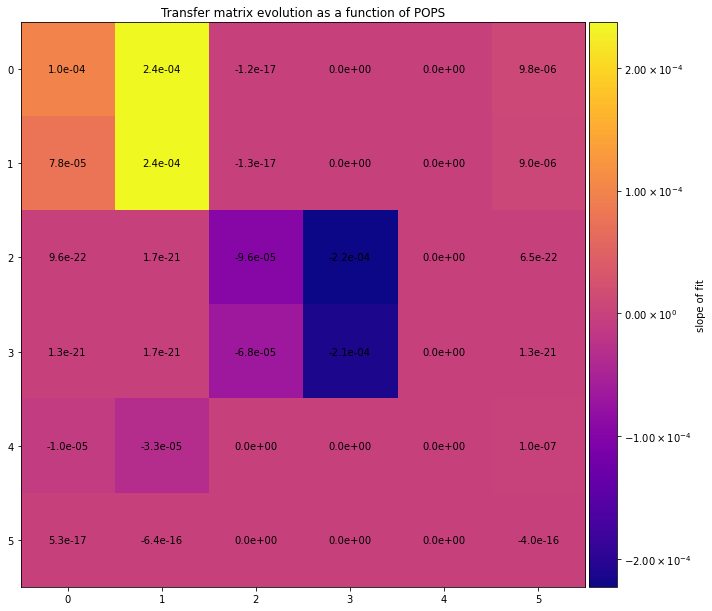
\includegraphics[width=1.0\textwidth]{02_Simulation/images/transfer_matrix_POPS.png}
\caption{Transfer matrix evolution as a function of POPS}
\label{fig:transfer_matrix_pops}
\end{figure}

The established transfer matrices can be utilized in MAD-X simulations to predict beam sizes under varying conditions. Notably, the elements \(R_{21}\), \(R_{22}\) (corresponding to \(p_{x,in}/x_{out}\) and \(p_{x,in}/p_{x,out}\)), and \(R_{34}\), \(R_{44}\) (corresponding to \(p_{y,in}/y_{out}\) and \(p_{y,in}/p_{y,out}\)) exhibited the most significant changes with variations in POPS, underscoring their critical role in beam dynamics at injection.


The source code for the simulations can be found in the following repositories:
\begin{itemize}
  \item \href{https://gitlab.cern.ch/eljohnso/acc-models-tls-eliott-fork/-/blob/EliottBranch/ps_injection/kick_response_injection_tracking/kick_response_BTP_injection_loop_transfer_matrix.ipynb}{Notebook: kick response BTP injection loop transfer matrix}
  \item \href{https://gitlab.cern.ch/eljohnso/acc-models-tls-eliott-fork/-/blob/EliottBranch/ps_injection/kick_response_injection_tracking/kick_response_BTP_injection_loop_transfer_matrix_function_of_POPS.ipynb}{Notebook: kick response BTP injection loop transfer matrix function of POPS.ipynb}
\end{itemize}


\subsection{Talk about how the shims are not implemented in OPERA and the solution in MAD-X}

\subsection{New chapter on extraction in F16}